\documentclass[a4paper,12pt]{report}

\usepackage[utf8]{inputenc}
\usepackage[T1]{fontenc}
\usepackage{array}
\usepackage{amsmath}
\usepackage[english]{babel}
\usepackage{bm}
\usepackage{graphicx}
\usepackage[a4paper]{geometry}
\usepackage[colorlinks=true,urlcolor=blue,linkcolor=blue]{hyperref}
\usepackage{url}
\usepackage[nottoc,numbib]{tocbibind}
\usepackage{color}
\usepackage{epstopdf}
\usepackage{xcolor}
\usepackage{rotating}
%\usepackage{wrapfig,booktabs}
\usepackage[backend=biber,style=phys]{biblatex}
\usepackage{upgreek}
\usepackage[capbesideposition={right,center}]{floatrow}

\addbibresource{../Bibliography.bib}

\makeatletter
	\renewcommand{\thechapter}{\Roman{chapter}}
\makeatother

\floatsetup[table]{style=plaintop}

\begin{document}

\chapter{Magneto-optical study of Cr-doped CdTe quantum dots\label{MagOptStud}}

%Plan:
%	Part I:
%		- On a vu du Cr. PL caractéristique en quatres pics, dont le second à plus haute énergie peut-être splitté. 
%		- Cr splitté par les contraintes bi-axiales. $S_z = \pm 2$ a assez haute énergie qu'ils ne peuvent pas être peuplé thermiquement. Raie splittée polaréisée linéairement correspond au 0.
%		- PL résolue en temps de la raie LE deux foiss plus longue que les autres -> peut correspondre à des dark exciton.
%		- Augmentation de la température -> pas d'apparition de $S_z = \pm 2$. De plus, $S_z = \pm 1$ disparaisse très rapidement => meilleure couplage aux noirs ?
%		- Bon couplage aux phonons optiques et accoustiques observé lors de la PLE.
%		- Etats avec une bonne conservation du spin observé dans la PLE.
%		- Magneto-optique confirme la structure énergétique. Plusieurs anti-crossing visible nous aide à identifier les états.
%		- La répartiton en intensité est compatible avec un couplage h-Cr anti-ferromaganétque. Cela peut-être du aux contrainted faisant bouger les niveaux du Cr et les bandes de CdTe.
%	Part II:
%		- Modèle de spin effectif prenant en compte la structure du Cr dans CdTe, l'interaction d'échange porteur-Cr et elecron-trou, l'effet Zeeman et le shift diamagnétique et le VBM reproduit bien effets observés expérimentalement. Une valeur de $D_0$ comprise entre 2 et 3 meV est déduite.
%		- Simulation de boîtes avec un fort E indique la possibilité d'observer de la polarisation linéaire sur toutes les raies. Pics peuvent ne pas être résolus -> pas trouvables pour nous (sélection de boîtes à faible E).
%	Part III:
%		- Boîtes trouvées présentant de la polar linéaire sur le trois raies. Mais magnéto-optique n'indique pas d'atome magnétique dedans. Evolution sous champs permets de changer le splitting.
%		- Hypothèse possible : Cr en dehors des boîtes. 3 états de charges possibles dans ZnTe => trois états pour la boîtes. Trou mal confiné peu avoir de l'overlap avec le Cr, mais chaque suivant état de charge du Cr.

	The main goal of this thesis was to include single Cr atoms in CdTe/ZnTe QDs. It was successfully achieved. We saw in Sec.~\ref{CrSemiCon} how the Cr atom is incorporated in II-VI semiconductor. We will now optically study Cr-doped QDs in order to probe the carrier-Cr interactions.
	
	We begin presenting the photoluminescence (PL) and the energy structure of the X-Cr complex. We show that the exchange interaction between the carrier and the Chromium is strong enough to see the effect of a single Cr spin in the quantum dots, giving the PL of the dots three characteristics peaks. We discuss the evolution of the emission in temperature and present different excited states of the system. Magneto-optical experiments confirm the energy structure, and suggests an anti-ferromagnetic coupling between hole and Cr spins. In the next section, we use the evolution of the QDs PL under magnetic field in order to deduce the QD parameters, using a spin hamiltonian model including the strain induced fine structure of the magnetic atom, the exchange coupling with the carriers and the influence of the reduced symmetry of the QDs on the electron-hole exchange interaction and on the valence band mixing. In the last section, we present dots having the characteristic three peaks PL, but that are not explained by our model. We finish proposing a possible explanation for those dots.

%	In this chapter, we will study the optical properties of a II-VI quantum dot containing a single Chromium atom. We saw in the Sec.~\ref{CrSemiCon} that the magnetic anisotropy of the spin leads to a zero magnetic field splitting of the $0$, $\pm 1$ and $\pm 2$ states. In a neutral Cr-doped quantum dot, such an anisotropy is induced by the bi-axial strains in the plane of the dots. Probing optically the dot, it results that exchange interaction is enough to see the effect of the presence of a single Cr spin in the QD. Studying the magnetic-field dependence of the quantum dots photoluminescence also shows the influence of the symmetry on carrier-Cr spin coupling.
%	
%	The chapter is organized as follows. First, we present the photoluminescence of several dots, extracting the X-Cr energy structure from it. Several features of this luminescence is then discussed. The study of the dot emission under magnetic field confirm the chosen energy structure. In the second section, we explain the model in more details, extracting parameters from the magneto-optics experiment, and examining its prediction for a different type of QD. Finally, we present and give a possible explanation to dots not explained by the model presented in this chapter.

	\section{Strained quantum dots containing an individual X-Cr atom}
	
		\subsection{Energy structure of X-Cr in a quantum dot~\label{CrPres}}
		
		Using the procedure described in Sec.~\ref{SKGrowth}, we randomly incorporated Cr atoms in CdTe/ZnTe quantum dots, adjusting the density of the Cr atoms to be roughly equal to the density of dots, in order to get QDs containing 0, 1 or a few Cr atoms. The photoluminescence (PL) of individual QDs, induced by optical excitation with a dye laser tuned on resonance with an excited state of the dots, is studied by optical micro-spectroscopy.
		
	\begin{figure}[h!]
	\begin{center}
		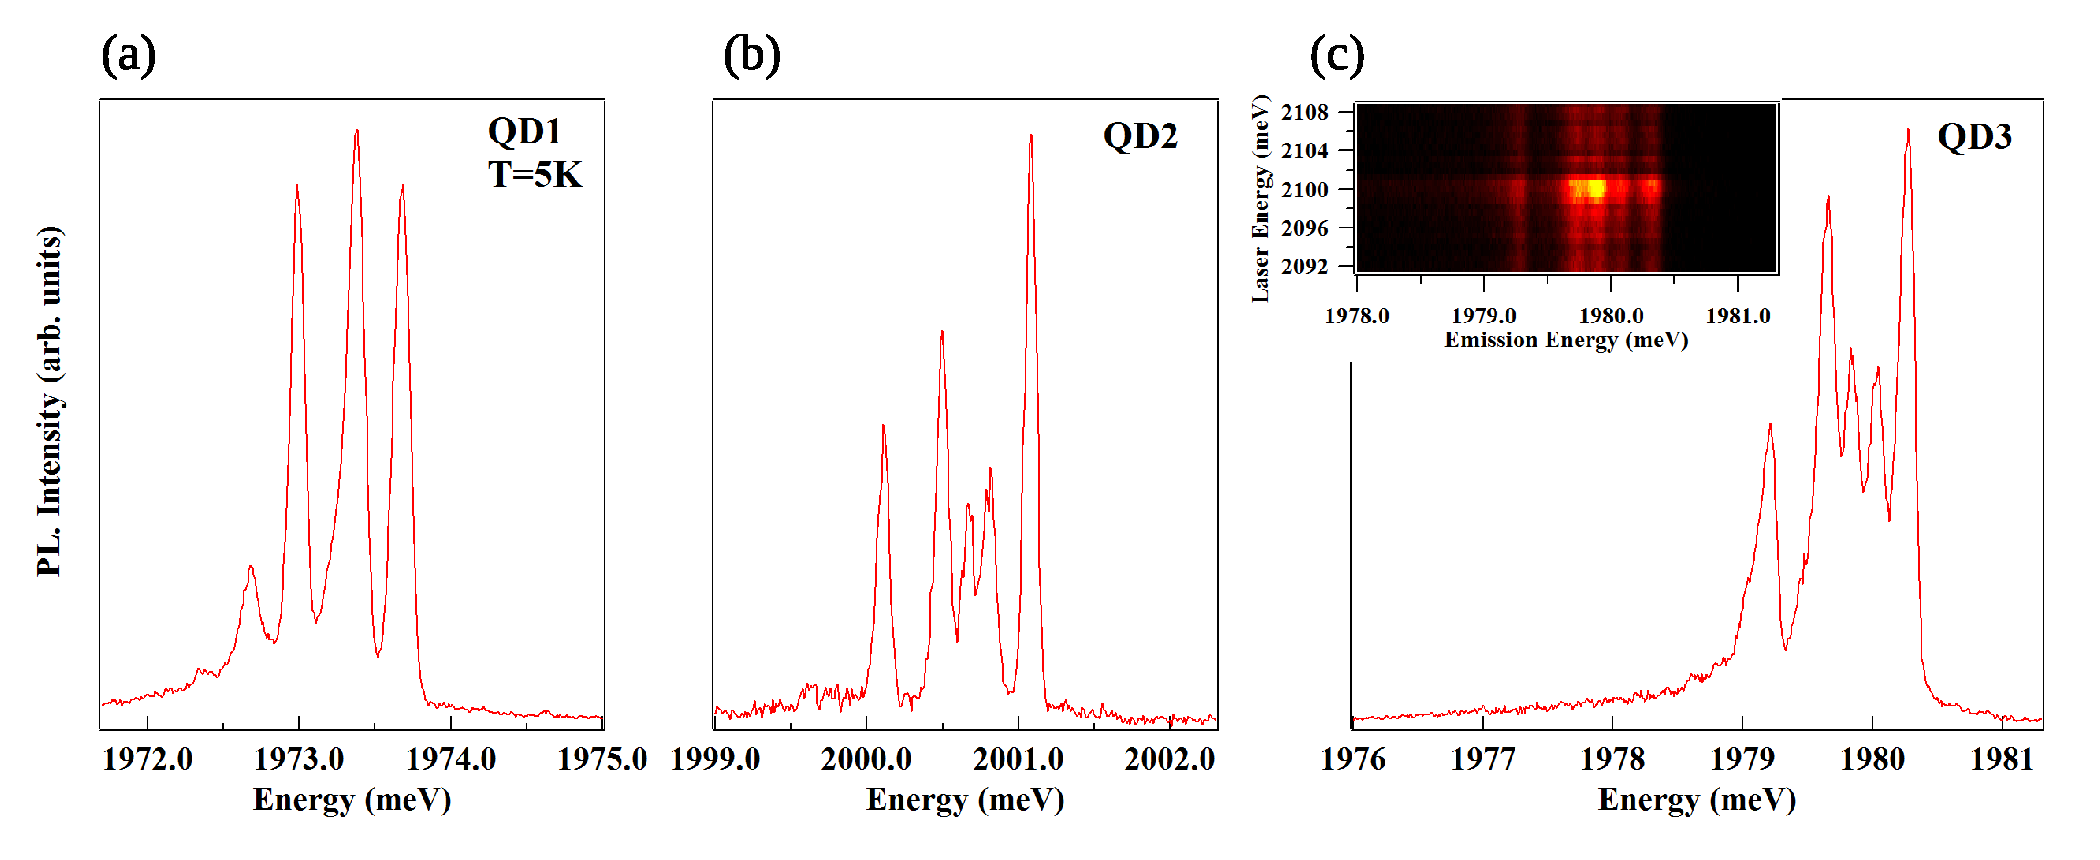
\includegraphics[width=15cm]{Pictures/Spectras.eps}
	\end{center}
	\caption{PL of (a) QD1, (b) QD2 and (c) QD3 X-Cr complex at low temperature (T=5K). Inset in (c) presents the PLE map of this QD, showing a sharp quasi-resonant state for an excitation at 2100 meV.}
	\label{SpectraX}
	\end{figure}

	Low temperature (T=5K) PL of the neutral exciton (X-Cr) of several QDs doped with a single Cr are reported in Fig.~\ref{SpectraX}. Characteristics three emission lines are observed, with a fourth, weaker peak on the low energy side. In some QDs, such as QD2 and QD3, the central peak was found to be split. Scanning with an energy tunable laser, we saw that all the peaks share a common excited state, as highlighted in the inset of Fig.~\ref{SpectraX}(c). This is an indication that they originate from the same dot. Variations in the relative intensities of the peaks are observed in different dots.

	\begin{figure}[h!]
	\begin{center}
		\includegraphics[width=10cm]{Pictures/EnLvlantiferro.png}
	\end{center}
	\caption{Illustration of the energy levels of the ground state (Cr), the bright exciton states ($|\pm1\rangle$) coupled to the spin of a Cr (X-Cr) and dominant PL transitions ($\sigma$+, $\sigma$-). The states $S_z = \pm2$ cannot be populated through thermalization, and thus their recombination channel are not shown on this schema.}
	\label{CrEnergyStruct}
	\end{figure}

	In a II-VI semiconductor, the orbital momentum of the Cr connects the spin of the atom to its local strain environment through the modification of the crystal field and the spin-orbit coupling. As we have seen in Sec.~\ref{CrSemiCon}, for biaxial strain in the (001) plane, the ground state of a Cr spin is split by a strain induced magnetic anisotropy term ${\cal H}_{Cr,\varepsilon_\parallel}=D_0S^2_z$. It was deduced from electron paramagnetic resonance of bulk Cr-doped CdTe that $D_0$ is positive for compressive biaxial strain~\cite{EPRCr}. In a self-assembled CdTe/ZnTe QDs with large in-plane strain, the Cr spin energy levels are split from $|S_z=0\rangle$ at low energy (Fig.~\ref{CrEnergyStruct}). A value of $D_0$ in the meV range can be expected for a CdTe layer strained on a ZnTe substrate, as shown in Sec.~\ref{CrSemiCon}.
	
	\begin{figure}[h!]
	\begin{center}
		\includegraphics[width=15cm]{Pictures/LinPol.png}
	\end{center}
	\caption{(a) Low temperature PL of QD2 recorded along two orthogonal directions. (b) Linear polarization PL intensity map of QD2. The 0$^{\circ}$ polarization angle corresponds to an emission polarized along the QD cleavage axis, either $[110]$ or $[1\bar{1}0]$. (c) Illustration of the energy levels of the ground state (Cr), the bright exciton states ($|\pm1\rangle$) coupled to the spin of a Cr (X-Cr), showing the splitting of the central peak via the bright exciton coupling, and dominant PL transitions ($\sigma$+ (blue), $\sigma-$ (red) and $\pi$ (green and black)).}
	\label{CrLinPolar}
	\end{figure}
	
	When an electron-hole pair is injected in a Cr-doped QD, the bright excitons are split by the exchange interaction between the spins of Cr and carriers. In flat self-assembled QDs, the heavy-holes and light-holes are separated in energy by the biaxial strain and the confinement. In a first approximation, the ground state in such QD is a pure heavy-hole ($J_z$=$\pm$3/2) exciton and the exchange interaction with the Cr spin S is described by the spin Hamiltonian 
	\begin{align}
		{\cal H}_{c-Cr}=I_{eCr}\mathbf{S}\cdot\bm{\upsigma}+I_{hCr}S_zJ_z
	\end{align}		
with $\bm{\upsigma}$ the electron spin and $J_z$ the hole spin operator. $I_{eCr}$ and $I_{hCr}$ are, respectively, the exchange integrals of the electron and the hole spins with the Cr spin. These exchange energies depend on the exchange constant of the Cr $3d$ electrons with the CdTe carriers and on the overlap of the Cr atom with the confined carriers. Even though the exchange interaction of the Cr spin with both electron and hole is ferromagnetic in most II-VI semiconductor~\cite{MacCdCrSD0beta,KacmanD0alphabetaIIVI,MacspdexchCr}, the hole-Cr interaction is supposed to be anti-ferromagnetic here. This does not change the structure of the PL at B = 0T. The only visible effect will be on the PL intensity distribution in the magneto-optics experiments. This will thus be further discussed in Sec.~\ref{MagOptCr}. A typical exchange constant 4 to 5 times larger for the holes than for the electrons is also expected in CdTe~\cite{DMSCrExchInt,CdCrSExchInt}.

	\begin{figure}[h!]
	\begin{center}
		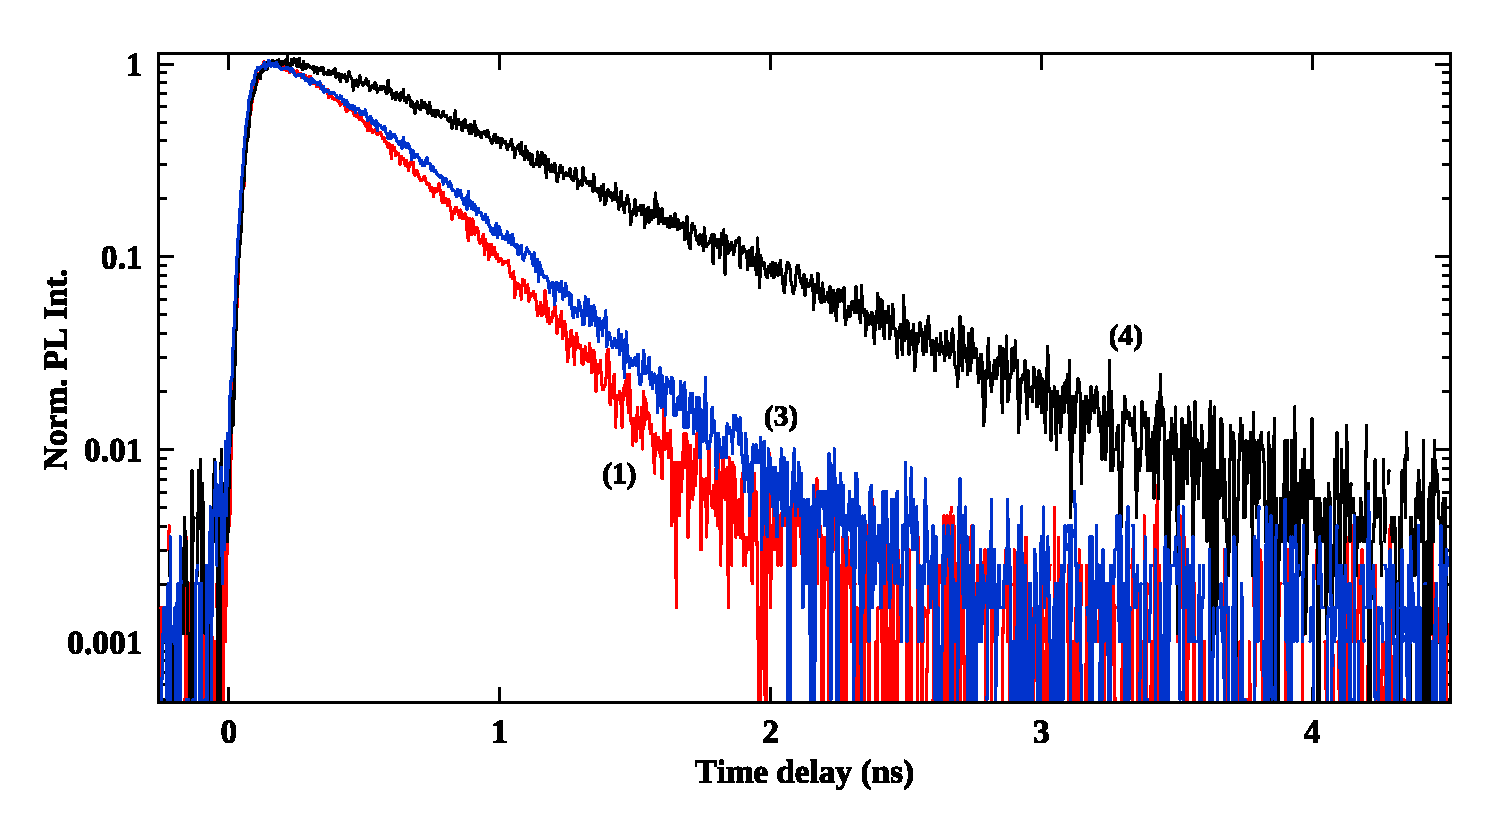
\includegraphics[width=12cm]{Pictures/Decay.eps}
	\end{center}
	\caption{Time resolved PL of QD2 taken on two outside peaks, attributed to $S_z = \pm1$ (noted (1) and (3) in Fig.~\ref{CrLinPolar}(a)), and the lower energy one (noted (4)).}
	\label{CrDecay}
	\end{figure}
	
	For highly strained CdTe/ZnTe QDs with a weak hole confinement, the strain induced energy splitting of the Cr spin $D_0S^2_z$ is much larger than the exchange energy with the confined carriers ($D_0\gg |I_{hCr}|>|I_{eCr}|$). The exchange interaction with the exciton acts as an effective magnetic field which further splits the Cr spins states $S_z=\pm$1 and $S_z=\pm$2. The resulting X-Cr energy levels are presented in Fig.~\ref{CrEnergyStruct}. The exciton recombination does not affect the Cr atom and its spin is conserved during the optical transitions. Consequently, the large strain induced splitting of the Cr spin is not directly observed in the optical spectra. However, at low temperature, the Cr spin thermalize on the low energy states $S_z$=0 and $S_z$=$\pm$1. This leads to a PL dominated by three contributions: a central line corresponding to $S_z=0$ and the two outer lines associated with $S_z=\pm$1 split by the exchange interaction with the carriers.
	
	Cr-doped quantum dots exhibit a linear polarization dependence, as presented in Fig.~\ref{CrLinPolar}. The central line ($S_z$=0) is split and linearly polarized along two orthogonal directions. As in non-magnetic QDs, this results from a coupling of the two bright excitons $|\pm1\rangle$ by (i) the long-range e-h exchange interaction in a QD with an in-plane shape anisotropy~\cite{SplitInvTh} and/or (ii) the short range e-h exchange interaction in the presence of valence band mixing. This anisotropic e-h exchange energy mixes the bright exciton associated with the same Cr spin state, inducing an extra splitting between them. The mixing is maximum for the central pair of bright excitons (S$_z$=0) which are initially degenerated. The outer lines are also slightly linearly polarized but the influence of the e-h exchange interaction is attenuated by the initial splitting of the $|\pm1\rangle$ excitons induced by the exchange interaction with the Cr spin $S_z=\pm1$.	

	In order to identify the lower energy peak ((4) in Fig.~\ref{CrLinPolar}(a)), we took the time resolved photoluminescence of the emission peaks, presented in Fig.~\ref{CrDecay}. One can notice that the line (4) present a decay time about twice longer than the one measured on the high energy peak. Such a long decay would be coherent with the radiative recombination of a dark exciton state. Under normal circumstances, the recombination of such a state is non-radiative. However, it is possible to observe a dark exciton recombination emitting a photon in low symmetry quantum dot~\cite{DELum}. Since it is initially a forbidden transition, the recombination will be less efficient and will thus take more time~\cite{DELongLifetime}. This hypothesis will be confirmed by the magneto-optical study of the dot presented in Fig.~\ref{CrMagOptExp} and \ref{CrMagOptMod}.
	
	\begin{figure}[h!]
	\begin{center}
		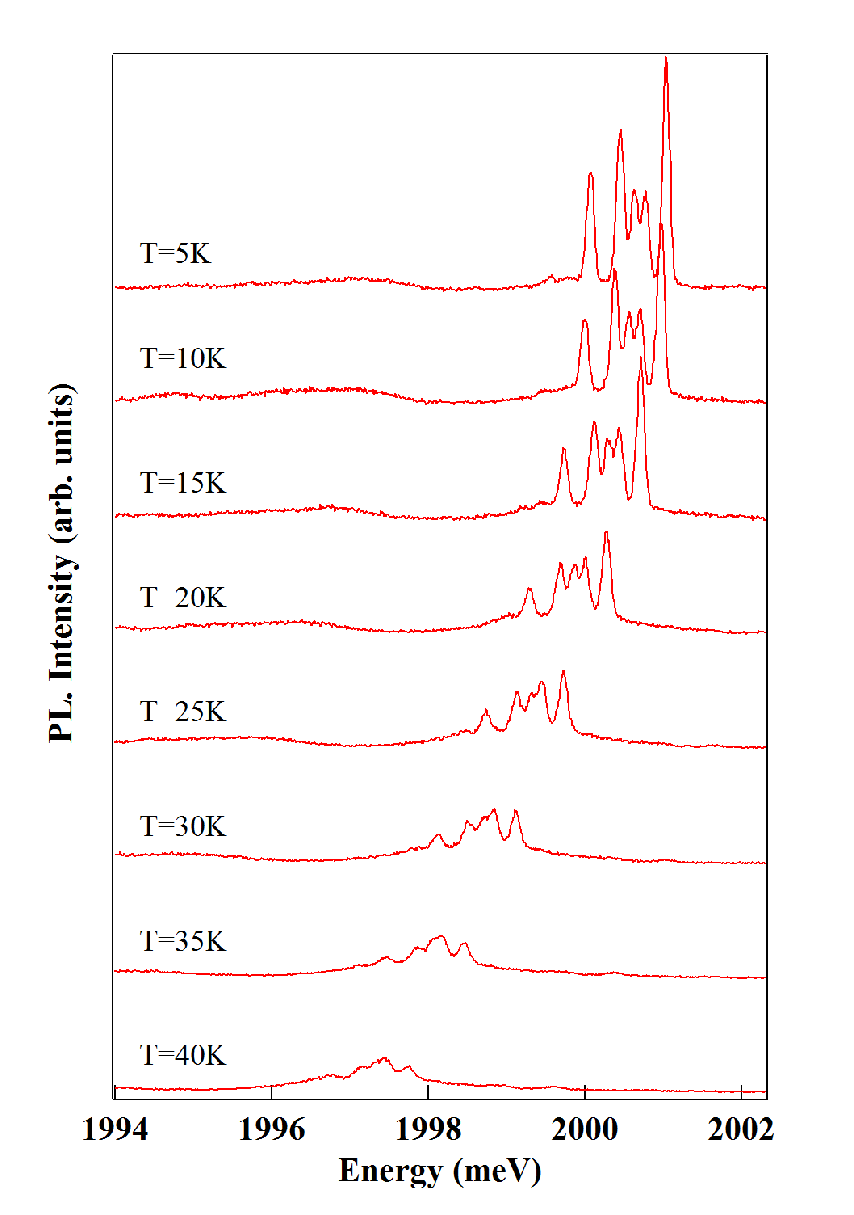
\includegraphics[width=14.9cm]{Pictures/Temp.eps}
	\end{center}
	\caption{Temperature evolution from T=5K to T=40K of (a) QD2 PL and (b) the PL of a QD with a good thermalisation on the low energy states (QD4). Even at 40K, $S_z = \pm2$ states do not appear.}
	\label{CrTemp}
	\end{figure}
	
	Since the Cr spin states $S_z = \pm2$ do not appear on the PL because they cannot be thermally populated at T = 5K, one could expect to see their emission at higher temperature. Fig.~\ref{CrTemp} presents the emission of two dots as a function of the temperature. With the increase of the temperature, we observe a significant line broadening induced by the interaction with acoustic phonons~\cite{BesombesAccPhon}. In order to keep a significant PL intensity and resolved PL lines, we limited our investigation to temperature below 40K. Even at this temperature, the $\pm2$ peak does not appear. However, the structure of the emission change slightly with the temperature. The intensity of the outside peaks, associated with the states $S_z = \pm1$, decreases while the emission of the $S_z = 0$ stays intense until higher temperature. This is an unexpected picture, since the temperature should allow the higher energy states $S_z = \pm1$ to be more populated by emptying the ground state. To explain this behaviour on the low energy peak, we propose that the states associated with the low energy transition are partly populated by the dark states. When the temperatures increase, the probability for the dark states to recombine non-radiatively increase, and thus the population and PL intensity of the low energy states would decrease.
	%\newpage

%	\begin{sidewaysfigure}
%	\begin{center}
%		\includegraphics[width=20cm]{Pictures/FullPLE}
%	\end{center}
%	\caption{(a) Map of QD2 PL under a scan in laser energy close to the dot emission in $\sigma -$ detection. Several interesting points are highlighted on zoom on each side of this whole map. (b) Map of the first few meV of the scan, showing the phonon replica. The emission integrated intensity in function of the laser energy is plotted in (c) (black curve) along with the PL spectra of QD2 (red curve). (d) - (f) present a zoom in a larger band at higher excitation energy in $\pi$,  $\sigma +$ and $\sigma -$ respectively. (g) Zoom on a particular excited state presented a splitting inversion, presented here in $\pi$ detection.}
%	\label{CrPLE}
%	\end{sidewaysfigure}

		\subsection{Excited states of a Cr-doped QD}	
	
	In order to study the different excited states in a QD doped with a single Cr atom, we took the PLE of QD2 starting close to the energy of the dot's emission. Fig.~\ref{FullPLE}(a) presents the entire PLE of QD2 X-Cr complex. One can note several excited states along the scan.
	
	\begin{figure}[h!]
	\begin{center}
		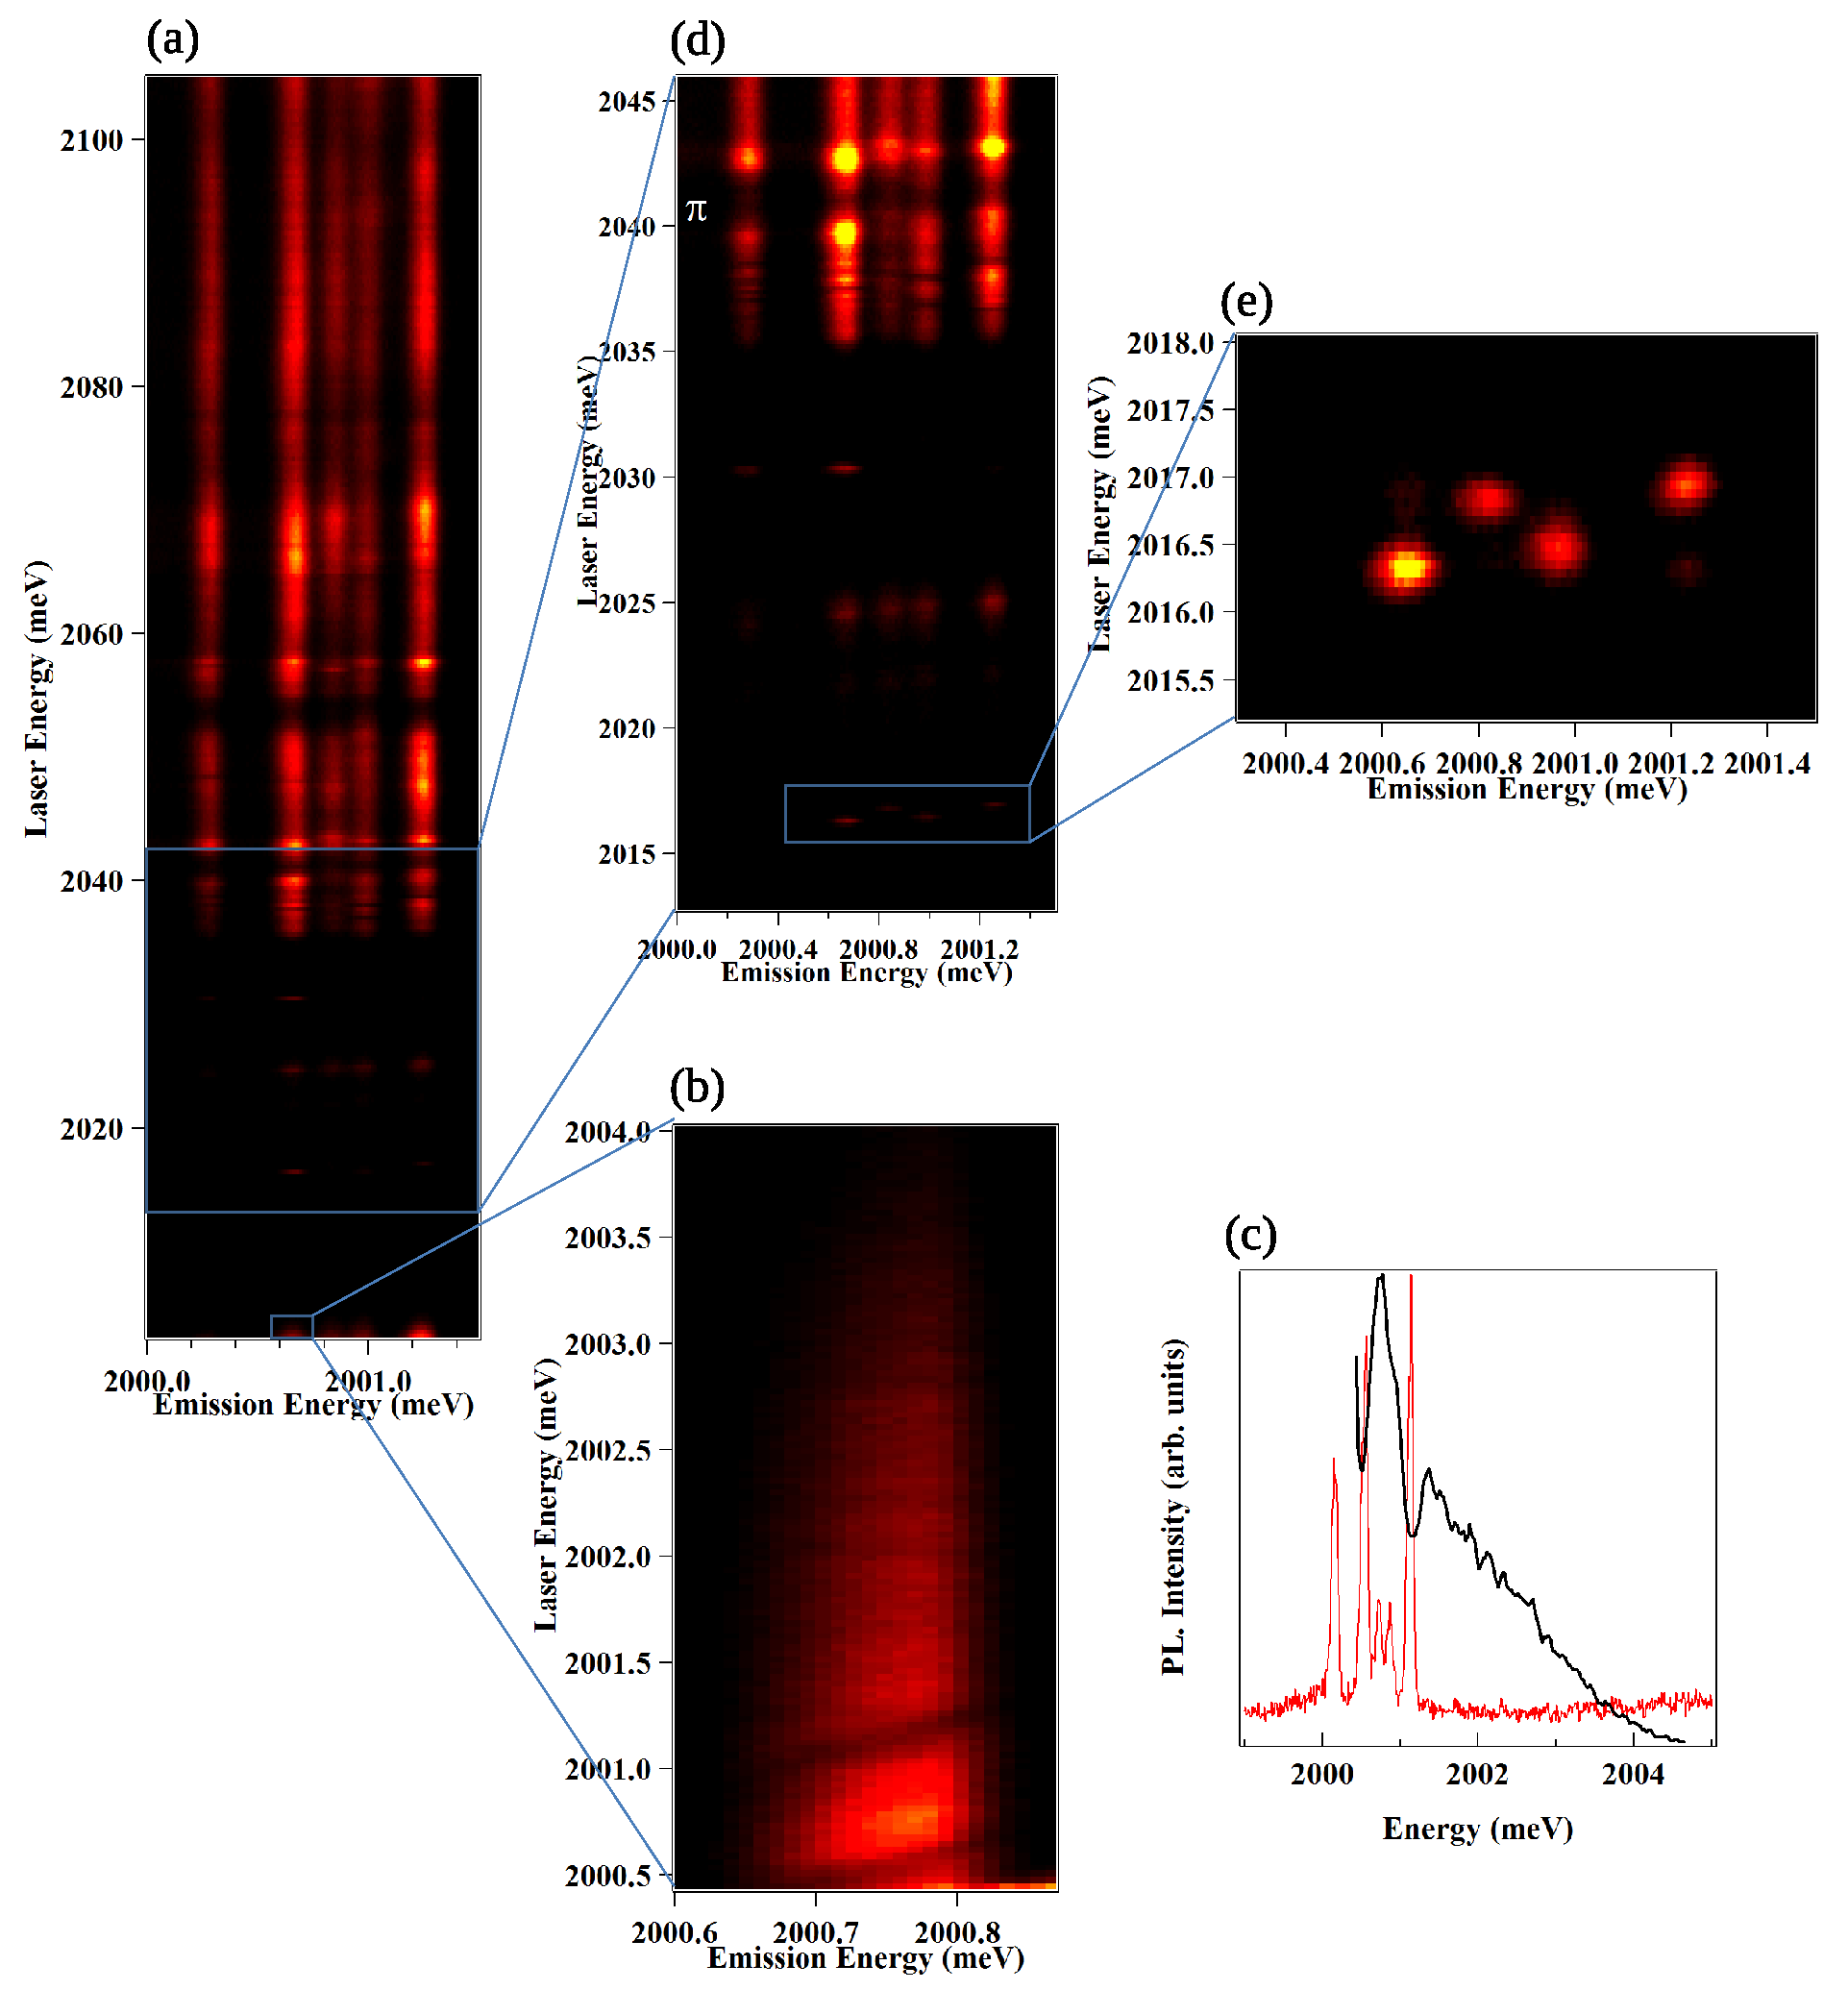
\includegraphics[width=13.8cm]{Pictures/FullPLEv2.eps}
	\end{center}
	\caption{(a) QD2 X-Cr PLE map in $\pi_{cross}$ polarization. Several excited states are highlighted. (b) Photoluminescence of QD2 X-Cr complex for an excitation at 2120 meV). (c) PLE scan detected on the lower energy peak, taken close to the QD emission energy, showing the phonon replica taken in $\pi$ detection. The emission integrated intensity in function of the laser energy is plotted in (d) (black curve) along with the PL spectra of QD2 taken in $\sigma_{co}$ polarization. (e) PLE map between 2046 meV and 2013 meV presenting several excited, detecting in $\pi_{cross}$ polarization. (f) Zoom in a particular excited state presented a splitting inversion, taken in $\pi_{cross}$ detection.}
	\label{FullPLE}
	\end{figure}
	
	The first remarkable feature of this scan is the luminescence over a large excitation energy range, for an excitation between the dot emission energy and 2004 meV. A zoom is presented in Fig.~\ref{FullPLE} (c) for a detection on the dark exciton line. This corresponds to an excitation of the QD via the acoustic phonon band. 
%	When on this band, the laser heat the sample, creating phonon in the absorption band on the dot.	The phonons will be able to excite the dot, generating an exciton inside and thus triggering the photoluminescence [A VERIFIER].
One can notice two sharp intensity decreases in this emission. Mapping the intensity of the phonon replica to the quantum dot spectrum (Fig.~\ref{FullPLE}(d)) show that they happen when the laser is in resonance with a QD emission line. The absorption then preferentially occurs in this resonantly excited state than in the acoustic phonon band of the low energy line.

%	\begin{figure}[h!]
%	\begin{center}
%		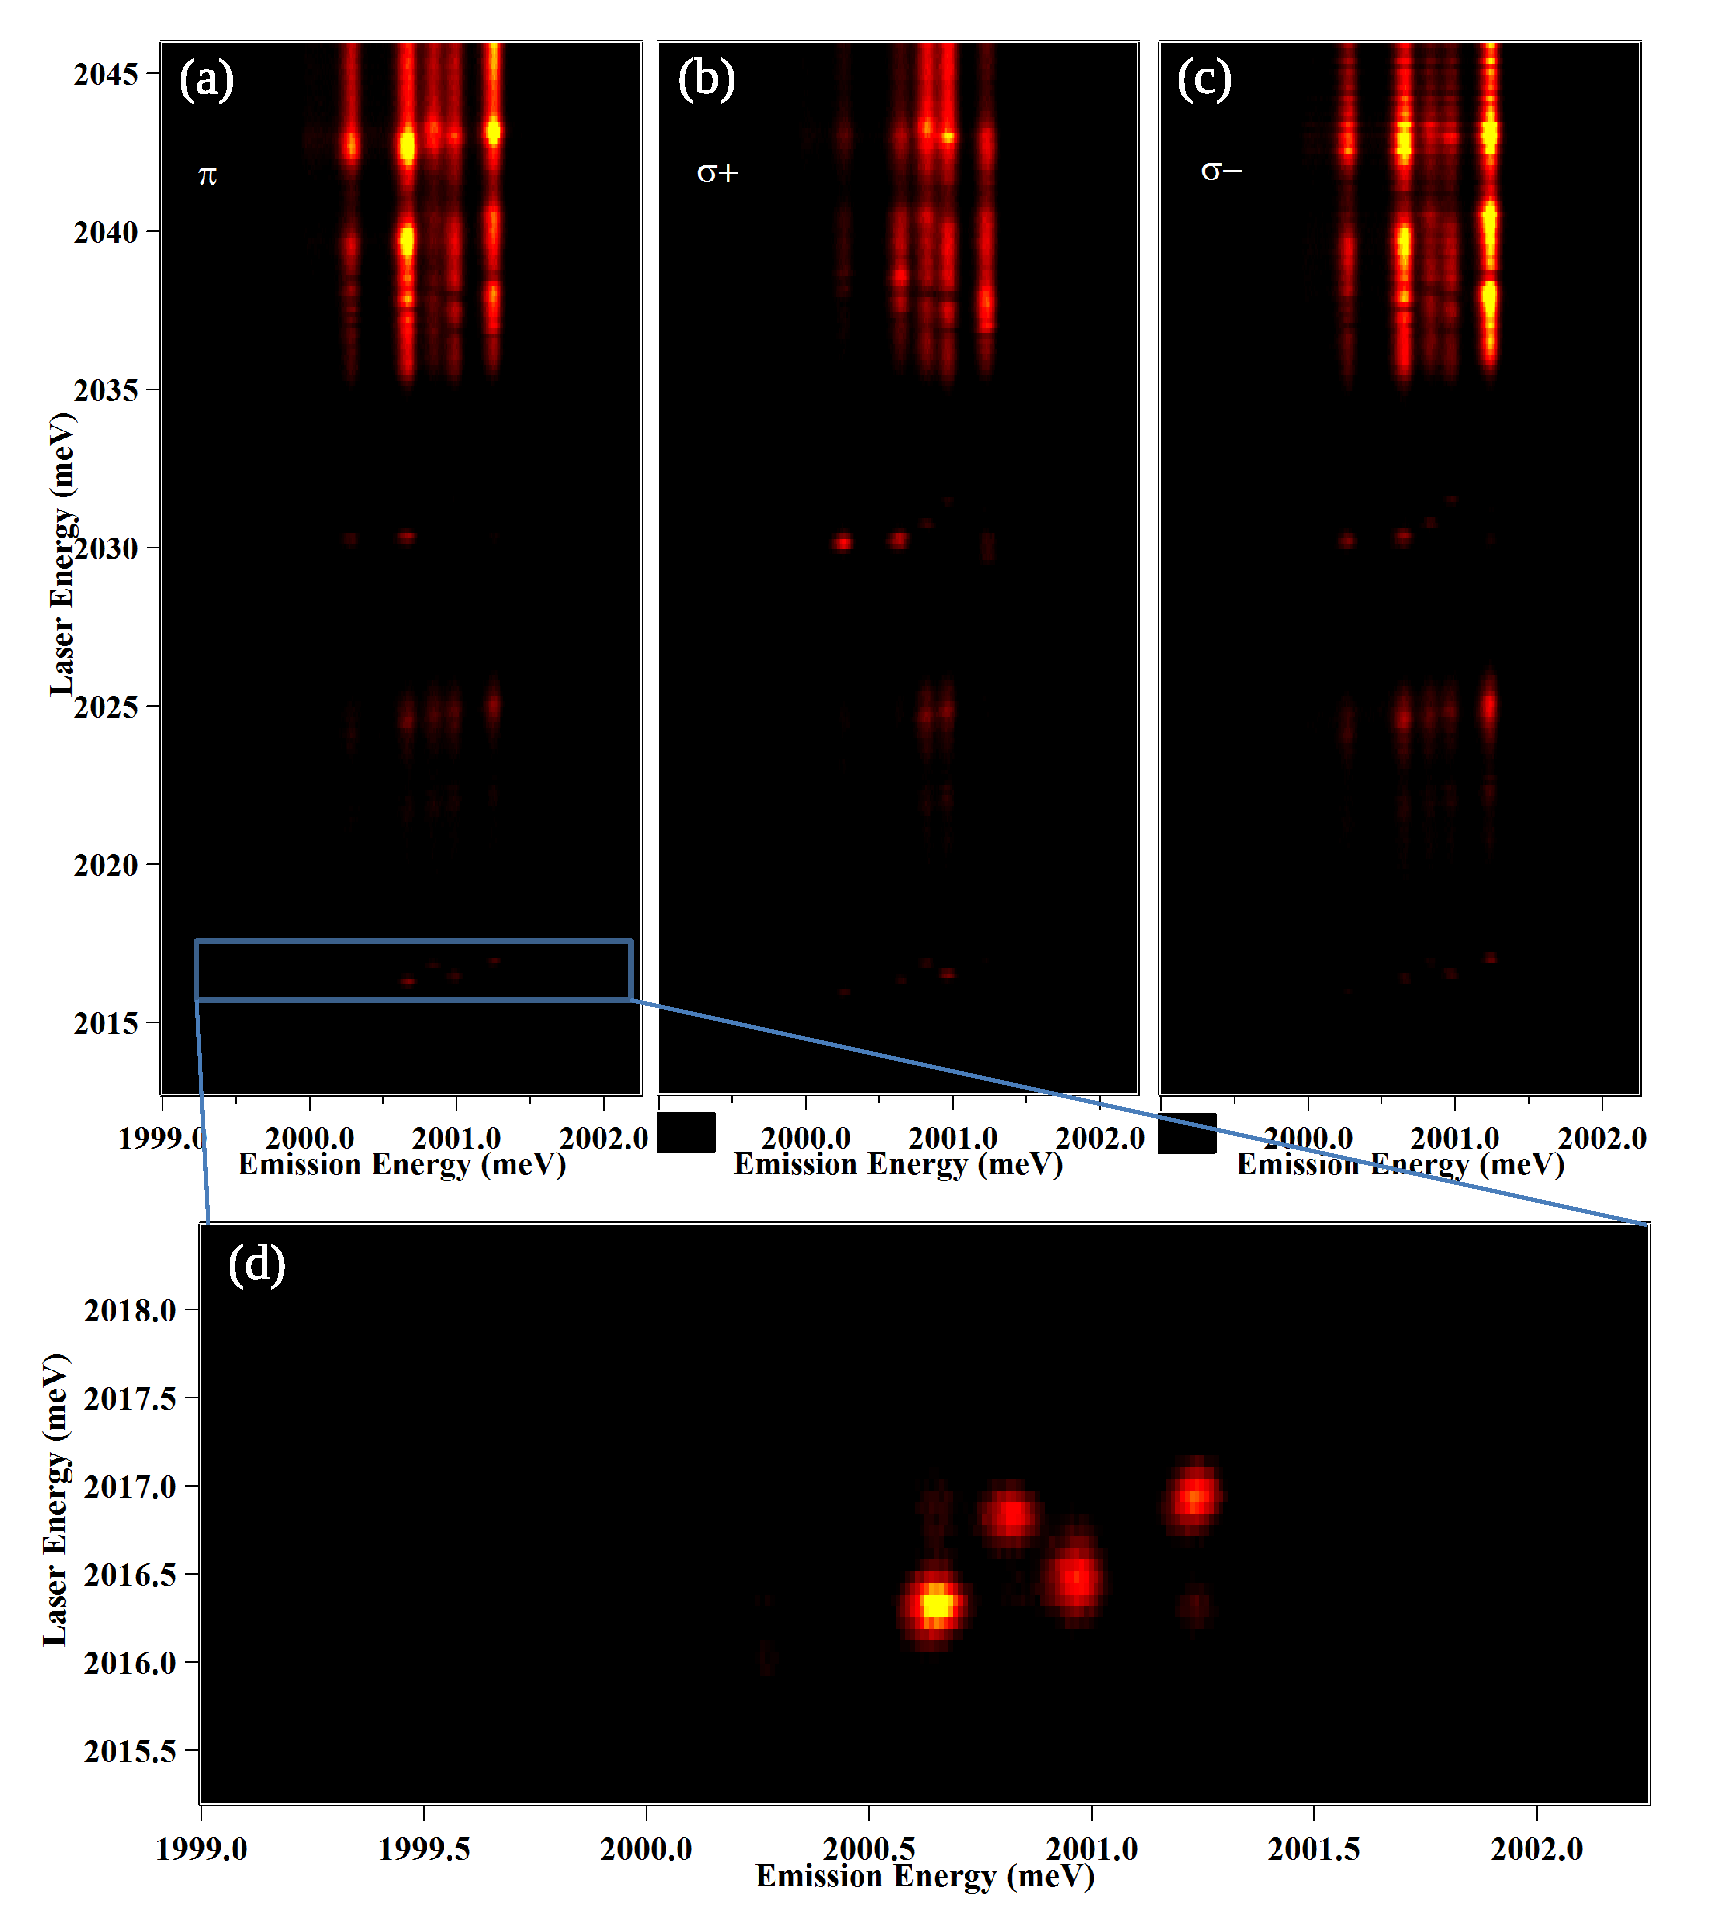
\includegraphics[width=12cm]{Pictures/PLE2030.eps}
%	\end{center}
%	\caption{(a) - (c) PLE map between 2046 meV and 2013 meV presenting several excited, detecting in $\pi$ (a),  $\sigma_{co}$ (b) and $\sigma_{cross}$ (c). (d) Zoom in a particular excited state presented a splitting inversion, taken in $\pi$ detection.}
%	\label{PLE2030}
%	\end{figure}
	
	Another excited state appear around 2018.5 meV, zoomed in on Fig.~\ref{FullPLE}(f). The first feature of this peak is that, each of the peak here presents a slightly different resonant energy. Moreover, one can note that the order of appearance of the two central peaks seems to be reversed compared to the external ones. Such splitting inversion, was first observed on QDs in GaAs quantum well~\cite{FineStructSplitGaAsdots}. It has been discussed by Takagahara~\cite{SplitInvTh} and is due to the electron-hole exchange interaction in anisotropic potential.
	
	\begin{figure}[h!]
	\begin{center}
		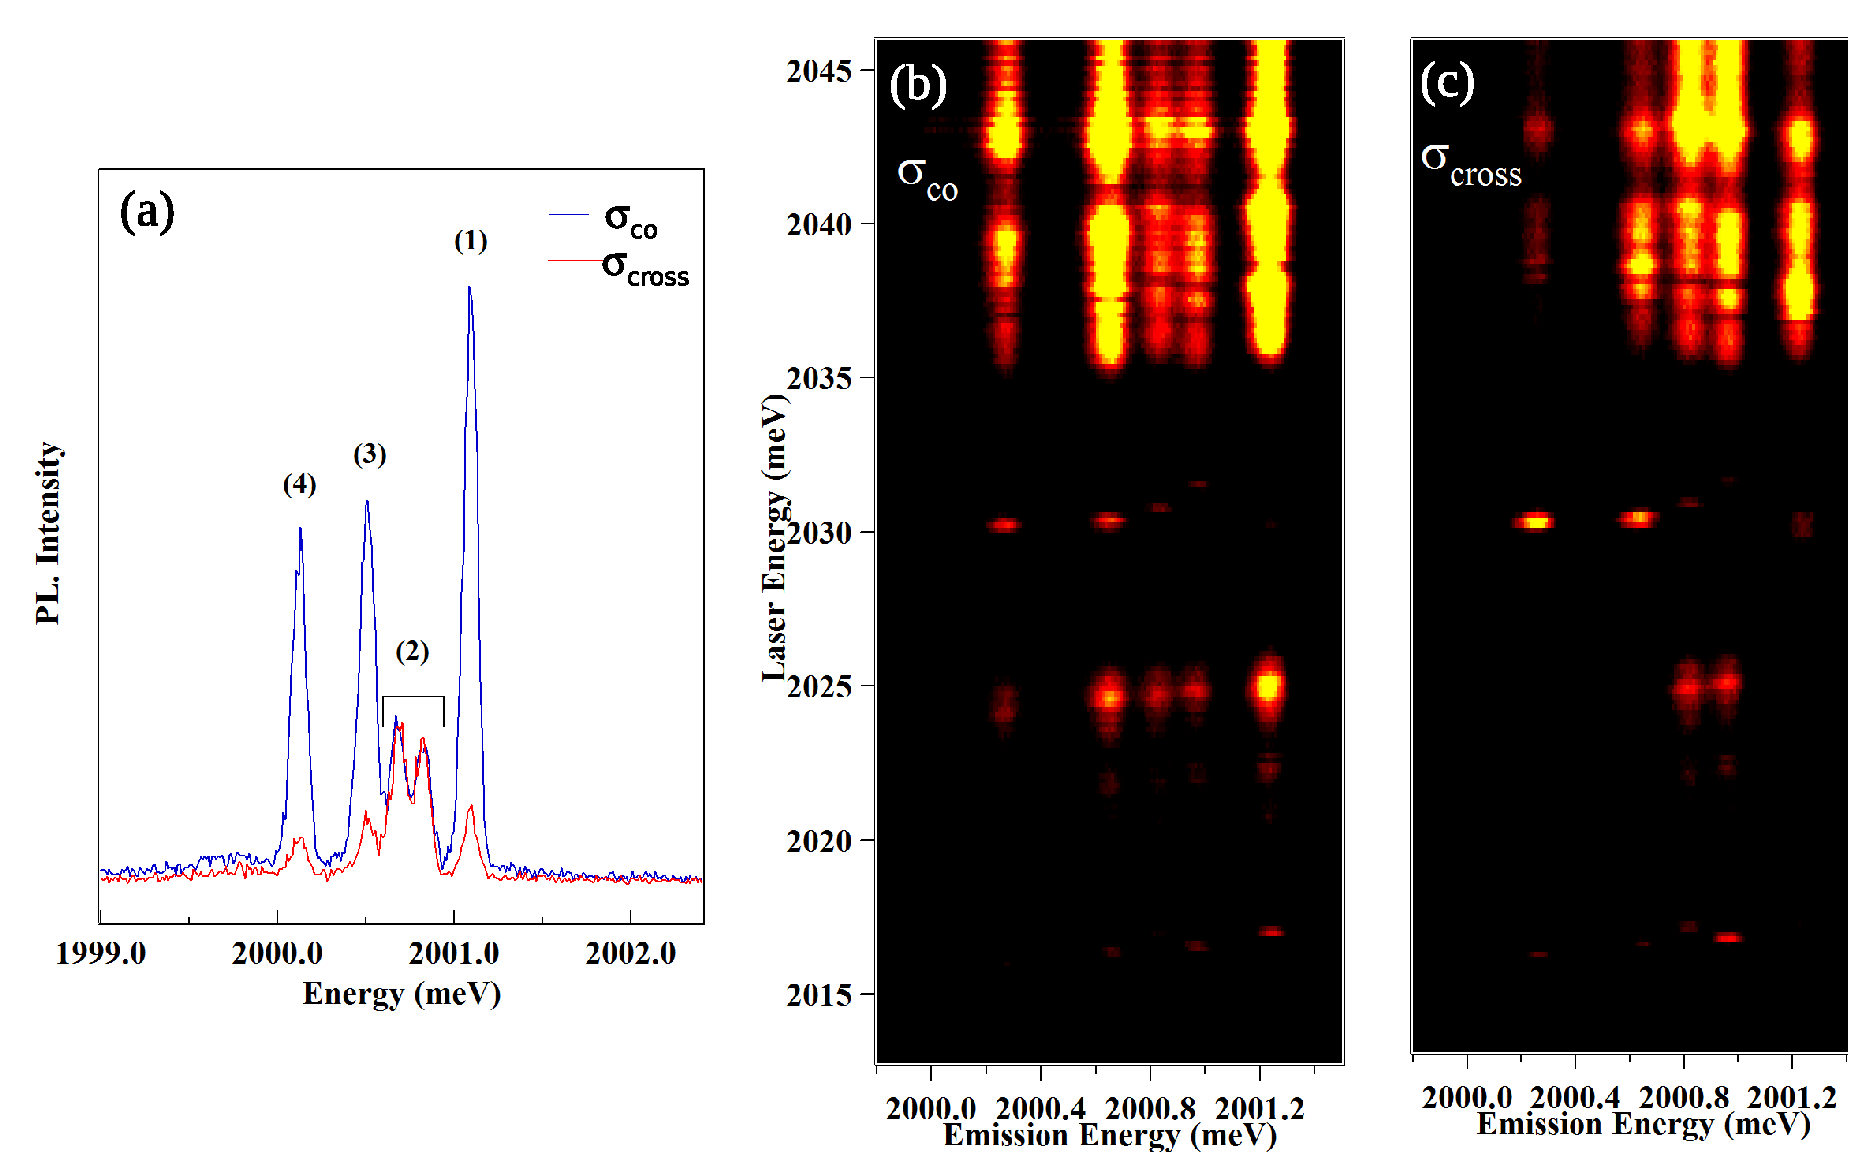
\includegraphics[width=14.9cm]{Pictures/PLEDotPres.eps}
	\end{center}
	\caption{(a) PL spectra of the exciton in QD2 (X-Cr) for co-circularly (blue) and cross-circularly (red) polarized excitation/detection taken for an excitation around 2120 meV. (b) - (c) PLE map between 2046 meV and 2013 meV presenting several excited states, detected in $\sigma_{co}$ (b) and $\sigma_{cross}$ (c).}
	\label{PLEDotPres}
	\end{figure}
	
	Another excited state can be seen at 2025 meV. It can be linked to an excitation through optical phonon. Looking at the $\sigma$ polarized emissions for an excitation on these states (Fig.~\ref{PLEDotPres}(b) and (c)), we can see that the low and high energy peaks are strongly $\sigma_{co}$ polarized. It means the exciton recombining is of the same spin as the one injected by the laser, and thus shows a good spin conservation of the exciton in the QD during its lifetime. This stabilization of the exciton spin is due to the Cr spin acting as an effective magnetic field on it. The split central peak emission is linearly polarized, as discussed in Sec.~\ref{CrPres}, and thus its emission shows no dependency in circular polarization. 
	
	Finally, another interesting excited state appear at 2030 meV. This state presents an exchange-induced splitting  different from the splitting in the excited state around 2120 meV presented in Fig.~\ref{SpectraX}. This difference is due to a difference in the carriers and Cr atom wavefunction overlap.

		\subsection{Magneto-optics of quantum dots doped with a single Cr atom\label{MagOptCr}}
		
	The structure of the energy levels in Cr-doped QDs is confirmed by the evolution of the PL spectra in magnetic field (up to 11T) along the growth axis, the so called Faraday configuration~\cite{BesombesPumpMnSFD}, presented in Fig.~\ref{CrMagOptExp}. Under magnetic field, the bright exciton $X_z = \pm1$ split, leading to a $\sigma-$ branch going at low energy and a $\sigma+$ one going at high energy. This splitting of the exciton under magnetic field can compensate the one induced by the exchange interaction with the Cr~\cite{LegerQDGeomEffect}. For QD1, this results in an anti-crossing of $|+1\rangle$ and $|-1\rangle$ excitons due to the e-h exchange interaction around B$_z$=6 T observed both in $\sigma+$ and $\sigma-$ polarizations (anti-crossing (2) and (3) in Fig.~\ref{CrMagOptExp}(a)).
		
	\begin{figure}[h!]
	\begin{center}
		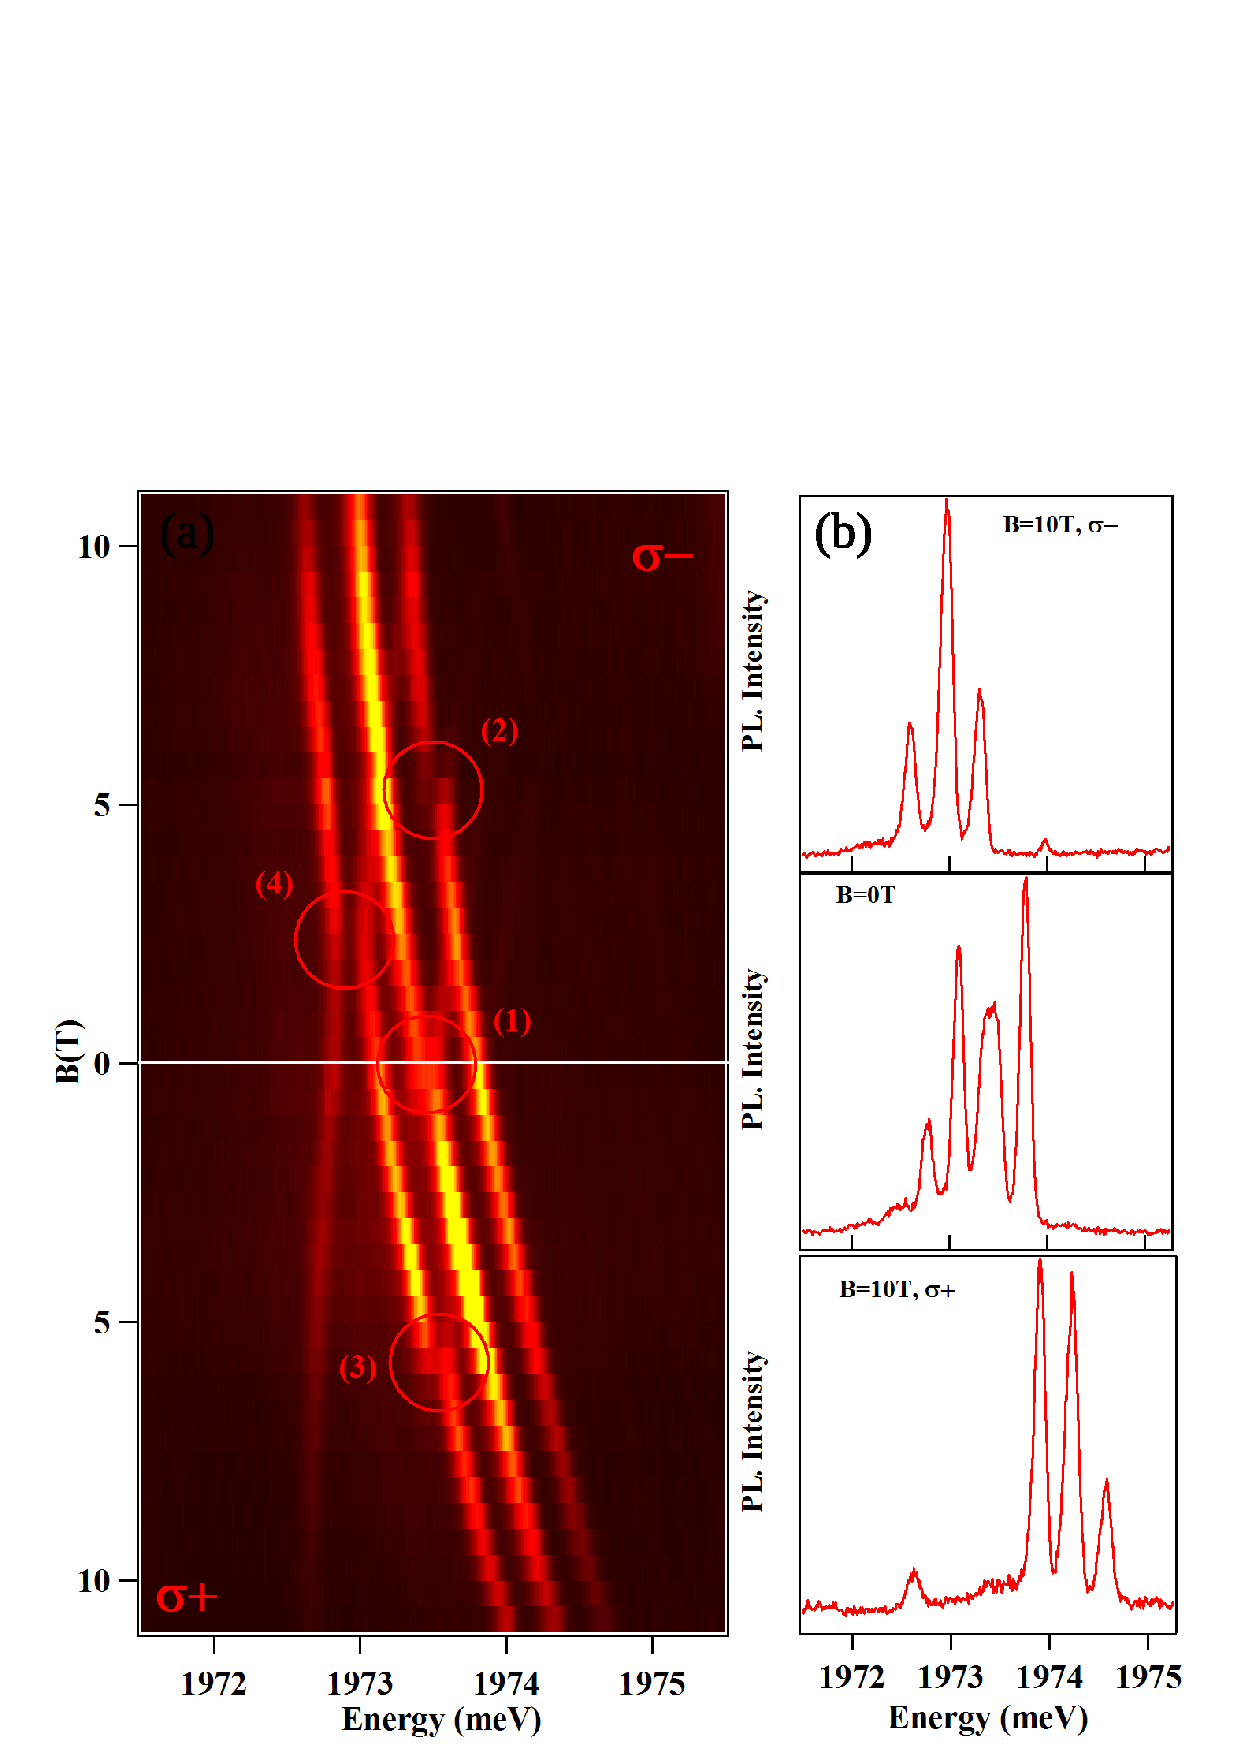
\includegraphics[width=10cm]{Pictures/MagOptv2.png}
	\end{center}
	\caption{(a) Circularly polarized X-Cr PL evolution under magnetic field ($B_z$) in QD1. Anti-crossings  are highlighted and numbered. (b) QD1 X-Cr PL spectra taken at 0 and $10$T for both circular polarization.}
	\label{CrMagOptExp}
	\end{figure}
		
		The low energy emission presented as a dark exciton in Fig.~\ref{CrDecay} shows an anti-crossing with the bright excitons under $B_z$ in $\sigma-$ polarization (anti-crossing (4) in Fig.~\ref{CrMagOptExp}). This anti-crossing arises from a mixing of the bright and dark excitons interacting with the same Cr spin state. Observed in $\sigma-$ polarization, it corresponds to the mixing of the exciton states $|-1\rangle$ and $|+2\rangle$ coupled to the Cr spin $S_z=+1$. This dark/bright excitons coupling $\delta_{12}$ is induced by the e-h exchange interaction in a confining potential of reduced symmetry (lower than C$_{2v}$)~\cite{DERecombTh}. In such symmetry, the dark exciton acquire an in-plane dipole moment which leads to possible optical recombination at zero magnetic field~\cite{DELum} as observed in these QDs. The oscillator strength of this "dark exciton" increases as the initial splitting between $|-1\rangle$ and $|+2\rangle$ excitons is reduced by the magnetic field.
		
	\begin{figure}[h!]
	\begin{center}
		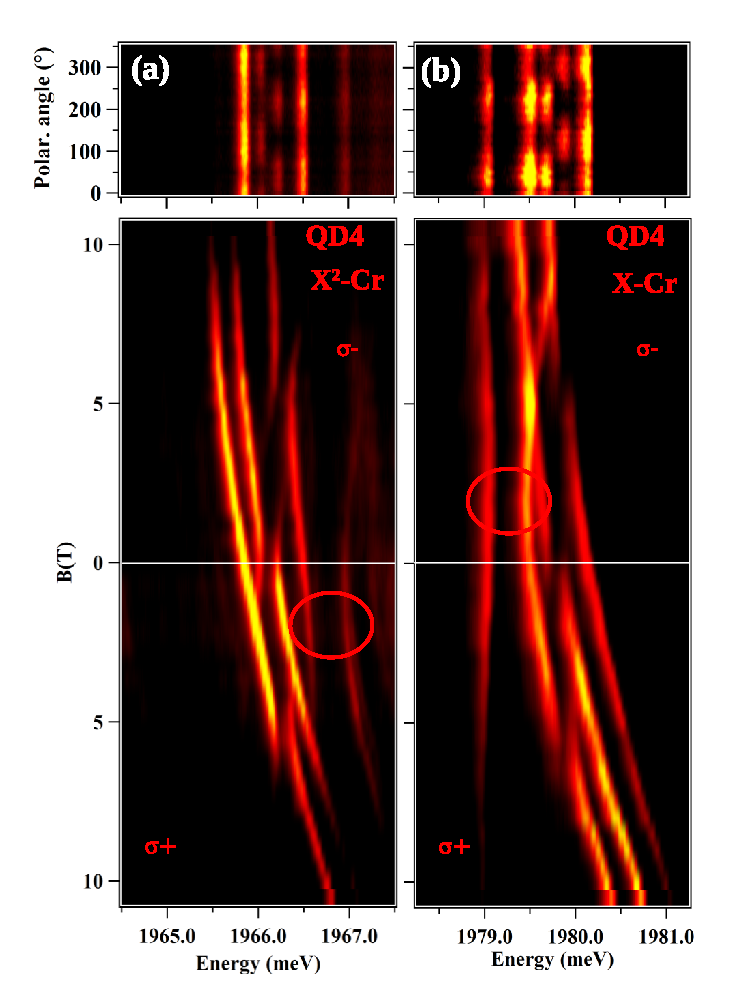
\includegraphics[width=10cm]{Pictures/MagOptLowSym.eps}
	\end{center}
	\caption{Linear polarization intensity map (top panel) and intensity map of the longitudinal magnetic field dependence of the emission (bottom panel) of (a) X$^2$-Cr and (b) X-Cr in QD3.}
	\label{CrMagOptLowSym}
	\end{figure}
		
		To illustrate the influence of the QD symmetry on the magneto-optical properties of X-Cr, we show in Fig.~\ref{CrMagOptLowSym}(b) the emission of a QD with a different strain or shape anisotropy (QD3). For QD1, the splitting of the central peak is not clear in the PL at 0T (Fig.~\ref{SpectraX}(a)), while two linearly polarized peaks appears clearly in QD3 spectra (Fig.~\ref{SpectraX}(c)).
%		This difference in emission arises from a difference in the in-plane strain anisotropy of each QD~\cite{SplitInvTh}.
		
		Investigating both the biexciton and the exciton in the same Cr-doped QD, we can also analyze the impact of the carrier-Cr interaction on the fine structure of the Cr spin. The magnetic field dependency of X$^2$-Cr emission in QD3 is presented along with the X-Cr emission as a contour plot in Fig.~\ref{CrMagOptLowSym}(a) and (b) respectively. The PL under magnetic field of X-Cr and X$^2$-Cr presents a mirror symmetry. In particular, the dark/bright exciton mixing observed around $B_z=2.5$ T on the low energy side of the PL in $\sigma-$ polarization for X-Cr is observed on the high energy side in $\sigma+$ polarization for X$^2$-Cr (circles in Fig.~\ref{CrMagOptLowSym}(a) and (b)).
		
	\begin{figure}[h!]
	\begin{center}
		\includegraphics[width=13cm]{Pictures/Antiferro-Cr.png}
	\end{center}
	\caption{(a) Evolution in magnetic field of QD4 X-Cr circularly polarized PL. (b) QD3 X-Cr PL at $B_z = 0$ T and $B_z = 7$ T in both polarization. A schema presenting the spin configuration for the most intense outer peak under magnetic field is joined on the side.}
	\label{CrAntiferro}
	\end{figure}
		
		If one consider the ground state of X$^2$ as a spin-singlet (total spin 0), it cannot be split by the magnetic field or the spin interaction part of the carriers-Cr hamiltonian. The creation of two excitons in the QD cancels the exchange interaction with the Cr atom. Thus, the PL of  X$^2$-Cr is controlled by the final state of the optical transitions, i.e. the eigenstates of X-Cr, resulting in the observed mirror symmetry in the PL spectra.
		
	\begin{figure}[h!]
	\begin{center}
		\includegraphics[width=10cm]{Pictures/Antiferro-Mn.eps}
	\end{center}
	\caption{(a) Evolution in magnetic field of the PL of a single Manganese atom coupled to an exciton in a II-VI QD. (b) PL spectra of the X-Mn system taken at $B_z = 0$ T and $B_z = 11$ T in both circular polarization. These experimental results are taken from Yoan L\'eger PhD thesis~\cite{YoanTh}.}
	\label{MnAntiferro}
	\end{figure}
		
	The evolution under magnetic field of the relative intensity of each of the QD peak gives information on the sign of the interaction between the Cr and the hole spin. As shown in Fig.~\ref{CrEnergyStruct}, given a polarization, each peak can be linked to a Cr spin state. As discussed earlier, applying a magnetic field lifts the degeneracy between the exciton states and allows to efficiently select the polarization of the emission. The evolution of the peaks relative intensities under magnetic thus gives information on the hole-Cr exchange interaction sign.
%	For QD1, as shown in Fig.~\ref{CrMagOptExp}, it is difficult to appreciate the variation of the relative intensity of the outside peaks. It hints for a high spin effective temperature, mediated by out of equilibrium phonons, allowing for high energy states to be populated.
	
	QD4, shown in Fig.~\ref{CrAntiferro}, presents a clear evolution of the intensity under magnetic field and will be used for this study. The central peak intensity stays the stronger of the three peaks, whatever the direction of the magnetic field. This is expected, since the $S_z = 0$ state is not affected by the Zeeman effect. It remains the lower spin state for the Cr atom, and therefore concentrate most of the population. In the $\sigma-$ branch, the high energy peak get brighter while the low energy one disappear for $B_z \geq 8$T in QD4. The situation is opposite in the $\sigma+$ branch, where the intensity concentrate on the lower energy peak.
	
	When applying a magnetic field, the Zeeman effect split the Cr spin states $S_z = \pm1$, with $S_z = -1$ going at lower energy and $S_z = +1$ going at higher energy. Therefore, at high enough magnetic field, the majority of the recombination will occur toward the $S_z = -1$. When exciting in $\sigma-$ polarization, we inject selectively exciton of total angular momentum $X_z = -1$. Since the high energy line is the only outer line remaining at high magnetic field, this means that the state $|S_z = -1, X_z = -1\rangle$ is at high energy. For an excitation in $\sigma+$ polarization, the injected exciton has an angular momentum $X_z = +1$ and the lower energy line is the most intense. It means the $|S_z = -1, X_z = +1\rangle$ state is at low energy. 

	This evolution is similar as the one observed in II-VI QDs doped by a single Mn atom, presented in Fig.~\ref{MnAntiferro} (from Yoan L\'eger PhD thesis~\cite{YoanTh}). Mn is known to have an anti-ferromagnetic interaction with the hole in CdTe~\cite{GajMnD0alphabeta}. It was shown in \cite{YoanTh} that, under magnetic field, the intensity was mainly on the high energy side when injecting $X_z = -1$ excitons, and on the low energy side when injecting $X_z = +1$ excitons. The structure is similar to the evolution of the PL of a Cr-doped QD under magnetic field.
	%The $S_z = -\frac{5}{2}$ state of the Mn atom was stabilized under magnetic field. From the evolution of the peaks relative intensity and the polarization of the different Mn states, it was then possible to deduce that the interaction between Mn and hole was anti-ferromagnetic.
%	
%	The evolution of the peaks relative intensity for the Cr looks like the one for the Mn. Under magnetic field, the $S_z = -1$ is stabilized, becoming the lower energy state of the doublet $S_z = \pm1$. For a high enough magnetic field, we can only consider the recombination toward $S_z = -1$. The high energy peak corresponds then to the $|S_z = -1, X_z = -1\rangle \rightarrow |S_z = -1\rangle$ on, emitting a $\sigma-$ polarized photon. The low energy one is associate with the $|S_z = -1, X_z = +1\rangle \rightarrow |S_z = -1\rangle$ transition, emitting a $\sigma+$ polarized photon. This is coherent with an anti-ferromagnetic coupling between the Cr and hole, contradicting the assumption made in Sec.~\ref{CrCdTe} and confirming the energy structure presented in Fig.~\ref{CrEnergyStruct}.

	All of this suggests an anti-ferromagnetic coupling between the Cr and the hole spins. It shows that the Cr spin interactions varies dramatically when inserted in a strain environment, as was discussed in Sec.~\ref{CrCdTe}. It also confirms the energy structure presented in Fig.~\ref{CrEnergyStruct}.
		
	\section{Modelization of a Cr-doped QD\label{QDParam}}
	
	We calculated the magneto-optic behaviour of Cr-doped QDs by diagonalizing the complete Hamiltonian of the e-h-Cr in self-assembled dots. We use for this purpose a spin effective hamiltonian that can be separated as follows:
	
	\begin{align}
\label{X-Cr} {\cal H}_{X-Cr}={\cal H}_{Cr,\varepsilon}+{\cal H}_{cCr}+{\cal H}_{mag}+{\cal H}_{eh}+{\cal H}_{band}+{\cal H}_{scat}
	\end{align}
where:

${\cal H}_{Cr,\varepsilon}$ describes the fine structure of the Cr atom and its dependency on local strain, as presented in Eq.~\ref{Cralone}. It is mainly drived by $D_0$, the magnetic anisotropy. E, the in-plane strain anisotropy, also appears in this Hamiltonian, but have to be kept small in order to model the found dots (see Fig.~\ref{CrHighE} for the emission of a dot with a higher E).

\begin{figure}[h!]
	\begin{center}
		\includegraphics[width=14.9cm]{Pictures/SimuAntiferro.png}
	\end{center}
	\caption{(a) Top: Calculated linear polarization PL intensity map of X-Cr at zero field. The 0$^{\circ}$ polarization angle correspond to an emission polarized along the $[100]$ axis. Bottom: Calculated X-Cr circularly polarized magnetic field dependency. Details of the model and parameters are listed in Tab.~\ref{CrModelParam}. Corresponding anti-crossing are highlighted in same fashion as on Fig.~\ref{CrMagOptExp} and \ref{CrAntiferro}. On the left, spectra calculated for $B_z = 0$ T and $B_z = 11$ T in both circular polarization are shown. The intensity was calculated using only thermal distribution. (b) Schema of the magnetic field dependency of the energy levels of the low energy Cr spin states $S_z$=0 and $S_z$=$\pm$1, and corresponding bright ($+1$ blue, $-1$ red) and dark ($|\pm2\rangle$ green) X-Cr energy levels.}
	\label{CrMagOptMod}
	\end{figure}

${\cal H}_{cCr}$ describes the coupling of the electron and hole with the Cr spin, depending on $I_{eCr}$, the exchange integral of the electron-Cr spins, and $I_{hCr}$, the exchange integral of the hole-Cr spins, as described in Eq.~\ref{HCrDMS}.

${\cal H}_{mag}$ describes the effect of a magnetic field, coupled to both the Cr and carrier spins by the Zeeman terms, depending on the $g$-factor of each of them and the Bohr magneton $\mu_B$, and including the diamagnetic shift of the electron-hole via the term $\gamma$.
\begin{align}
	{\cal H}_{mag} = g_{Cr}\mu_B\overrightarrow{B}.\overrightarrow{S}+g_{e}\mu_B\overrightarrow{B}.\overrightarrow{\sigma}+g_{h}\mu_B\overrightarrow{B}.\overrightarrow{J}+\gamma B^2
\end{align}

${\cal H}_{eh}$ describes the short range and long range electron-hole interaction, through the bright and dark exciton splitting $\delta_0$, the bright exciton coupling $\delta_1$, the dark exciton coupling $\delta_2$ and the bright and dark exciton coupling $\delta_{11}$ and $\delta_{12}$. All of these term are described in Eq~\ref{HehCs}.

${\cal H}_{band}$ is the band Hamiltonian. It is written ${\cal H}_{band} = E_g + {\cal H}_{VBM}$, with $E_g$ the CdTe gap energy and ${\cal H}_{VBM}$ is described in Eq.~\ref{HVBM}.

${\cal H}_{scat}$ describes the perturbation of the wave function of the exciton in the initial state of the optical transition by the hole-Cr exchange interaction, controlled by the parameter $\eta$. It was found to be essential to explain the dynamic of X$^+$-Mn and is introduced here for generality purpose. This perturbation depends on the value of the exchange energy between the Cr spin $S_z$  and the hole spin $J_z$ and can be represented, using second order perturbation theory, by an effective spin Hamiltonian \cite{CarInSpinSplit,BiexFinStruct,DynhMn}
\begin{align}
{\cal H}_{scat}=-\eta S_z^2
\end{align}
\noindent with $\eta>0$.

	We considered the general case of QDs with a symmetry lower than C$_{2v}$ (truncated ellipsoidal lens for instance~\cite{DERecombTh}), and took into account the influence of this reduced symmetry on the valence band and on the e-h exchange interaction. The population of the X-Cr spin states split by the large magnetic anisotropy and the carriers-Cr exchange interaction is described by a spin effective temperature $T_{eff}$, applied on the X-Cr levels. The results of the model obtained with $T_{eff}=$20K, $D_0=2.2$ meV and an electron-Cr (hole-Cr) exchange interaction $I_{eCr}=-50$ $\mu$eV ($I_{hCr}=250$ $\mu$eV) are reported in Fig.~\ref{CrMagOptMod} (parameters not specific to Cr-doped QDs are listed in Tab.~\ref{CrModelParam}). Such parameters do not aim to precisely fit the data and are only reasonable order of magnitude to qualitatively reproduce the experimental results of the PL of X-Cr at zero field and its evolution in magnetic field. The splitting of the central line at zero field (anti-crossing (1)) and the anti-crossings under magnetic field (anti-crossings (2) and (3) around $B_z$=6T for the Cr spin states  $S_z = |+1\rangle$ and anti-crossings (4) with the dark exciton around $B_z$=2T) are well reproduced by the model.
	
	This model also predicts an anti-crossing around $B_z = 5$ T, noted (5), caused by an electron-Cr flip flop, which is not seen on the experiments. Its position is controlled by $D_0$ and its intensity by $I_{eCr}$. However, for this anti-crossing to appear for $B_z > 11$T, a $D_0 > 3$ meV is needed, causing the $S_z = \pm1$ levels to be at high energy and thus giving a stronger emission intensity to the $S_z = 0$ state than the one sawn experimentally. Therefore, a low value of $I_{eCr}$ was chosen instead. Finally, the remaining tail of an anti-crossing, labelled (6), also appears at high magnetic field in the $\sigma-$ polarization, as seen in Fig.~\ref{CrAntiferro}, due to the coupling a bright and a dark exciton coupled to the Cr state $S_z = 0$.

	
%	\begin{table}[t] \centering
%	\caption{Values of the parameters used in the model of Cr-doped CdTe/ZnTe quantum dot presented in Fig.~\ref{SpectraX}(b). The value of the parameters not listed in the table is 0. The chosen values are typical for CdTe/ZnTe quantum dots and can be compared with parameters extracted from Mn-doped quantum dots \cite{DynhMn,DELum}. These values are reasonable to reproduce the emission of the QDs presented in this thesis.}
%	\renewcommand{\arraystretch}{1.0}
%	\begin{tabular}{p{0.9cm}p{0.9cm}p{0.9cm}p{0.9cm}p{0.9cm}p{0.9cm}p{0.9cm}p{0.9cm}p{0.9cm}p{0.9cm}p{0.9cm}p{0.9cm}p{0.9cm}p{1.3cm}
%p{0.9cm}p{0.9cm}}
%\hline\hline
%I$_{eCr}$ & I$_{hCr}$ & $\delta_0$ & $\delta_1$ & $\delta_{12}$ & $\delta_{11}$ & $\frac{|Q|}{\Delta_{lh}}$ & $\frac{|R|}{\Delta_{lh}}$ & arg(R) & $D_0$ & $g_{Cr}$ & $g_{e}$ & $g_{h}$ & $\gamma$ & $\eta$ & $T_{eff}$ \\
%$\mu eV$ & $\mu eV$ & $meV$ & $\mu eV$ & $\mu eV$ & $\mu eV$ &  & & & $meV$ & &  &  & $\mu eV/T^2$ & $\mu eV$ & K \\
%\hline
%-70 & -280 & -1 & 250 & 150 & 50 & 0.05 & 0.05& $-\frac{\pi}{2}$ & 2.5 & 2 & -0.7 & 0.4 & 1.5 & 25 & 25 \\
%\hline\hline 
%	\end{tabular}
%	\label{CrModelParam}
%	\end{table}

%\begin{wraptable}{r}{5.5cm}
%	\caption{Values of the parameters used in the model of Cr-doped CdTe/ZnTe quantum dot presented in Fig.~\ref{SpectraX}(b). The value of the parameters not listed in the table is 0. The chosen values are typical for CdTe/ZnTe quantum dots and can be compared with parameters extracted from Mn-doped quantum dots \cite{DynhMn,DELum}. These values are reasonable to reproduce the emission of the QDs presented in this thesis.}
%	\renewcommand{\arraystretch}{1.0}
%	\begin{tabular}{m{1.3cm}|m{1.3cm}||m{1.3cm}}
%I$_{eCr}$ & $\mu eV$ & -70\newline \\
%I$_{hCr}$ & $\mu eV$ & -280\newline \\
%$\delta_0$ & $meV$ & -1\newline \\
%$\delta_1$ & $\mu eV$ & 250\newline \\
%$\delta_{12}$ & $\mu eV$ & 150\newline \\
%$\delta_{11}$ & $\mu eV$ & 50\newline \\
%$\frac{|Q|}{\Delta_{lh}}$ &  & 0.05\newline \\
%$\frac{|R|}{\Delta_{lh}}$ &  & 0.05\newline \\
%arg(R) &  & $-\frac{\pi}{2}$\newline \\
%$D_0$ & $meV$ & 2.5\newline \\
%$g_{Cr}$ &  & 2\newline \\
%$g_{e}$ &  & -0.7\newline \\
%$g_{h}$ &  & 0.4\newline \\
%$\gamma$ & $\mu eV/T^2$ & 1.5\newline \\
%$\eta$ & $\mu eV$ & 25\newline \\
%$T_{eff}$ & K & 25\newline \\
%	\end{tabular}
%	\label{CrModelParam}
%	\end{wraptable}

\begin{table}[t] \centering
	\caption{Values of the parameters used in the model of Cr-doped CdTe/ZnTe quantum dot presented in Fig.~\ref{CrMagOptMod}. The value of the parameters not listed in the table is 0. The chosen values are typical for CdTe/ZnTe quantum dots and can be compared with parameters extracted from Mn-doped quantum dots \cite{DynhMn,DELum}. These values are reasonable to reproduce the emission of the QDs presented in this thesis.}
	\renewcommand{\arraystretch}{1.0}
	\begin{tabular}{p{0.9cm}p{0.9cm}p{0.9cm}p{0.9cm}p{0.9cm}p{0.9cm}p{0.9cm}p{0.9cm}}
\hline\hline
I$_{eCr}$ & I$_{hCr}$ & $\delta_0$ & $\delta_1$ & $\delta_{12}$ & $\delta_{11}$ & $\frac{|s|}{\Delta_{lh}}$ & $\frac{|r|}{\Delta_{lh}}$ \\
$\mu eV$ & $\mu eV$ & $meV$ & $\mu eV$ & $\mu eV$ & $\mu eV$ &  & \\
\hline
-50 & 250 & -1 & 250 & 150 & 50 & 0.05 & 0.05 \\
\hline\hline 
	\end{tabular}
	\begin{tabular}{p{0.9cm}p{0.9cm}p{0.9cm}p{0.9cm}p{0.9cm}p{1.3cm}p{0.9cm}p{0.9cm}}
arg(r) & $D_0$ & $g_{Cr}$ & $g_{e}$ & $g_{h}$ & $\gamma$ & $\eta$ & $T_{eff}$ \\
 & $meV$ & &  &  & $\mu eV/T^2$ & $\mu eV$ & K \\
\hline
$-\dfrac{\pi}{2}$ & 2.2 & 2 & -1 & 0.4 & 1.5 & 25 & 20 \\
\hline\hline
	\end{tabular}
	\label{CrModelParam}
	\end{table}
	
	The magnetic anisotropy $D_0$ cannot be precisely extracted from the PL spectra. However, for $D_0 <  2$ meV, an anti-crossing due to a VBM induced hole-Cr flip-flop between the $|-1, +2\rangle$ and the $|0, -1\rangle$ would appear below $B_z=11$ T on the central line in $\sigma-$ polarization. Moreover, as discussed earlier, a $D_0 > 3$ meV would produce a lower PL intensity for the states $S_z = \pm1$. These consideration sets a $D_0$ in the range of 2 to 3 meV. However, even in this range, the intensity distribution of the PL cannot be perfectly reproduced: while the evolution under magnetic field of the intensity ratio of the peaks is quite well predicted for high value of the magnetic field, the $S_z = 0$ state still presents a stronger emission at $B_z = 0$ T than the one observed in the experiments. This difference in intensity may be due to out of equilibrium phonons in the sample that help populating the $S_z = \pm1$ states.

	Our model reproduce qualitatively with enough satisfaction the data found experimentally and thus can be used to see the evolution of the emission varying different parameters. Especially, an interesting point is the influence of the anisotropy of strains on the emission. The results of the calculations are presented on Fig.~\ref{CrHighE}. The QD emission at 0 T splits into six ilnes with the same linear polarization dependency. The contrast gets higher with the in plane strain anisotropy.
	
	\begin{figure}[h!]
	\begin{center}
		\includegraphics[width=13cm]{Pictures/HighE.eps}
	\end{center}
	\caption{Calculated X-Cr linear polarization intensity map at B = 0T (top) and circularly polarized magnetic field dependency (bottom) for dot with an anisotropy of strains (a) $E = 25$ $\mu$eV and (b) $E = 100$ $\mu$eV. Anti-crossings numbered (1) to (6) are still there, but are not highlighted for the sake of clarity.}
	\label{CrHighE}
	\end{figure}
	
	As discussed previously, the in-plane anisotropy couples two states close in energy and separated by two units of spin. This is the case of the states $S_z = +1$ and $S_z = -1$ for the Cr atom. A small anisotropy of strain term $E$ cannot couple those states, and thus they do not present linear polarization in QD with a low in-place anisotropy. Increasing the value of the anisotropy make it possible for these levels to be coupled, giving their emission a linear polarization dependency. On the magnetic field map of the PL, this appears as anti-crossing at B = 0 T, noted (9) and (10) on Fig.~\ref{CrHighE}.

	Two other anti-crossings appears when putting a higher in plane anisotropy term $E$. They appear on the low and high energy peaks, around B = 4 T and are numbered (7) and (8) on Fig.~\ref{CrHighE}. They occur when the states $|S_z = +1, X_z = -1\rangle$ and $|S_z = -1, X_z = -1\rangle$ are brought together by the Zeeman effect. These states are composed of two Cr spin states separated by two units of spin coupled to the same exciton state. They are then coupled by the anisotropy term $E$ when bought at the same energy by the magnetic field.

	Fig.~\ref{CrHighE} (b) shows the evolution of linear polarization intensity map and the circularly polarized magnetic field dependency of a Cr-doped QD with a higher $E$ value. We can see that the contrast of the linear polarization is stronger, while the anti-crossings are wider and occur on a larger range of energy. A higher in-plane strain anisotropy term $E$ is able to couple the states on a wider range of energy before and after they are actually brought in degeneracy. These wider anti-crossings overlap and lead to an apparent diminution of the peaks splitting at zero magnetic field.
%	For a higher value of $E$, the anti-crossings are wider. They occur on a larger range of energy, and  with a wider split for the anti-crossing (8) and (9). This leads to a superposition of the different anti-crossing, giving a complex magnetic dependency and the apparent reduction of the splitting at B = 0 T.
	
	Most of the dot we found presented a small anisotropy term $E$. The reason might be a selection bias. The splitting at zero magnetic field leads to a spectra with six different peaks. Moreover, we saw on Fig.~\ref{CrHighE} (b) that the splitting at B = 0T can be reduced due to the width of the anti-crossings. The resolution of our monochromator might then not be precise enough to resolve the peaks, and only shows a broad emission. Such a dot would then not be selected for further studies, leading to a selection bias toward low anisotropy dots.
	
	\section{Charge fluctuation of a Cr ion  in the vicinity  of the QDs\label{ChargeFluc}}
	
	Some dots were found presenting a linear polarization dependency all their peaks, for both X-Cr and X$^2$-Cr. One of them, QD5, is presented on Fig.~\ref{CrSixPeaksMagOpt}. Such a dependency is expected in dots with a strong in-plane anisotropy term $E$, as shown in Sec.~\ref{QDParam}. While a thin and well resolve X$^+$-Cr is observed on all these dots, X-Cr is often not resolved, appearing as a broad emission. Such a result was also expected for dots with a large $E$.
	
	\begin{figure}[h!]
	\begin{center}
		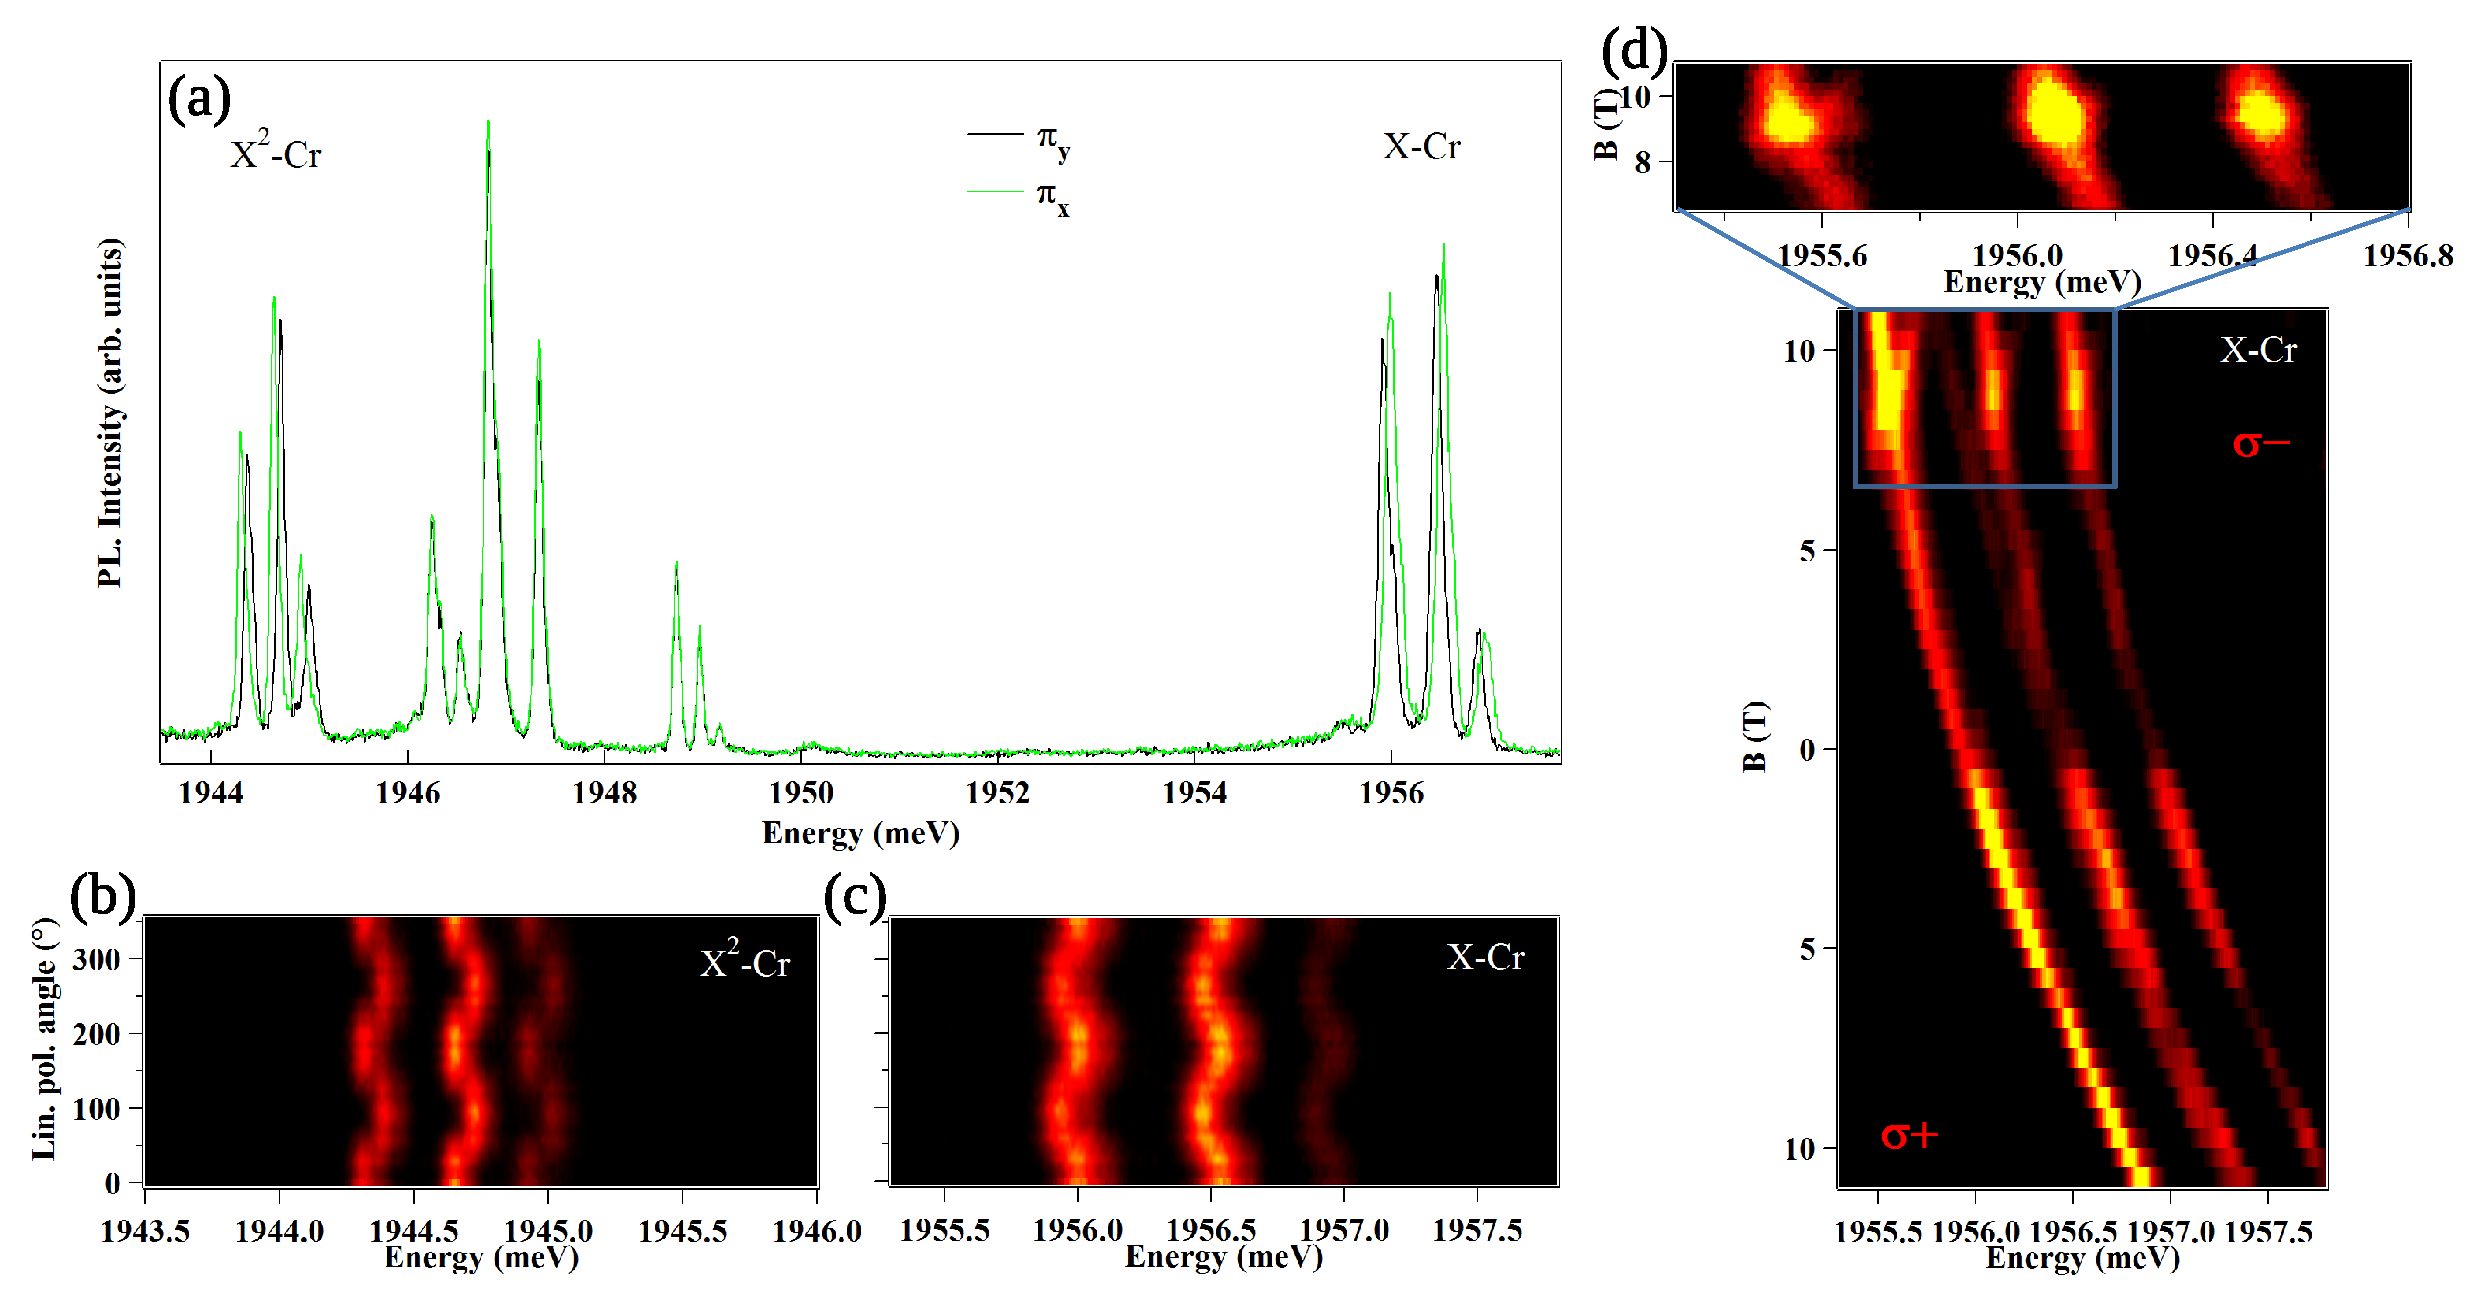
\includegraphics[width=14.9cm]{Pictures/6peaks.eps}
	\end{center}
	\caption{(a) QD5 linearly polarized PL intensity at zero magnetic field. (b) and (c) Respectively QD5 X$^2$-Cr and X-Cr linear polarization PL dependence at zero magnetic field. (c) X-Cr magnetic field PL dependence of QD5. Zoom in presents anti-crossing appearing at B=9T.}
	\label{CrSixPeaksMagOpt}
	\end{figure}
	
	However, studying the dot under magnetic field show no appearance of the expected anti-crossing for a QD with a high $E$. The dots present a single anti-crossing on all their peaks for B = 9T in $\sigma-$ polarization. This is characteristic of the mixing between bright and dark exciton as observed in non-magnetic QDs. The complex behaves like three non-magnetic QDs emitting at close energy. However, all the peaks were found to have the maximum intensity for the same position on the sample, and they share excited states on the PLE. It is highly improbable to find three dots close to each other, emitting almost at the same energy and sharing excited states at several position on the sample.

	\begin{figure}[h!]
	\begin{center}
		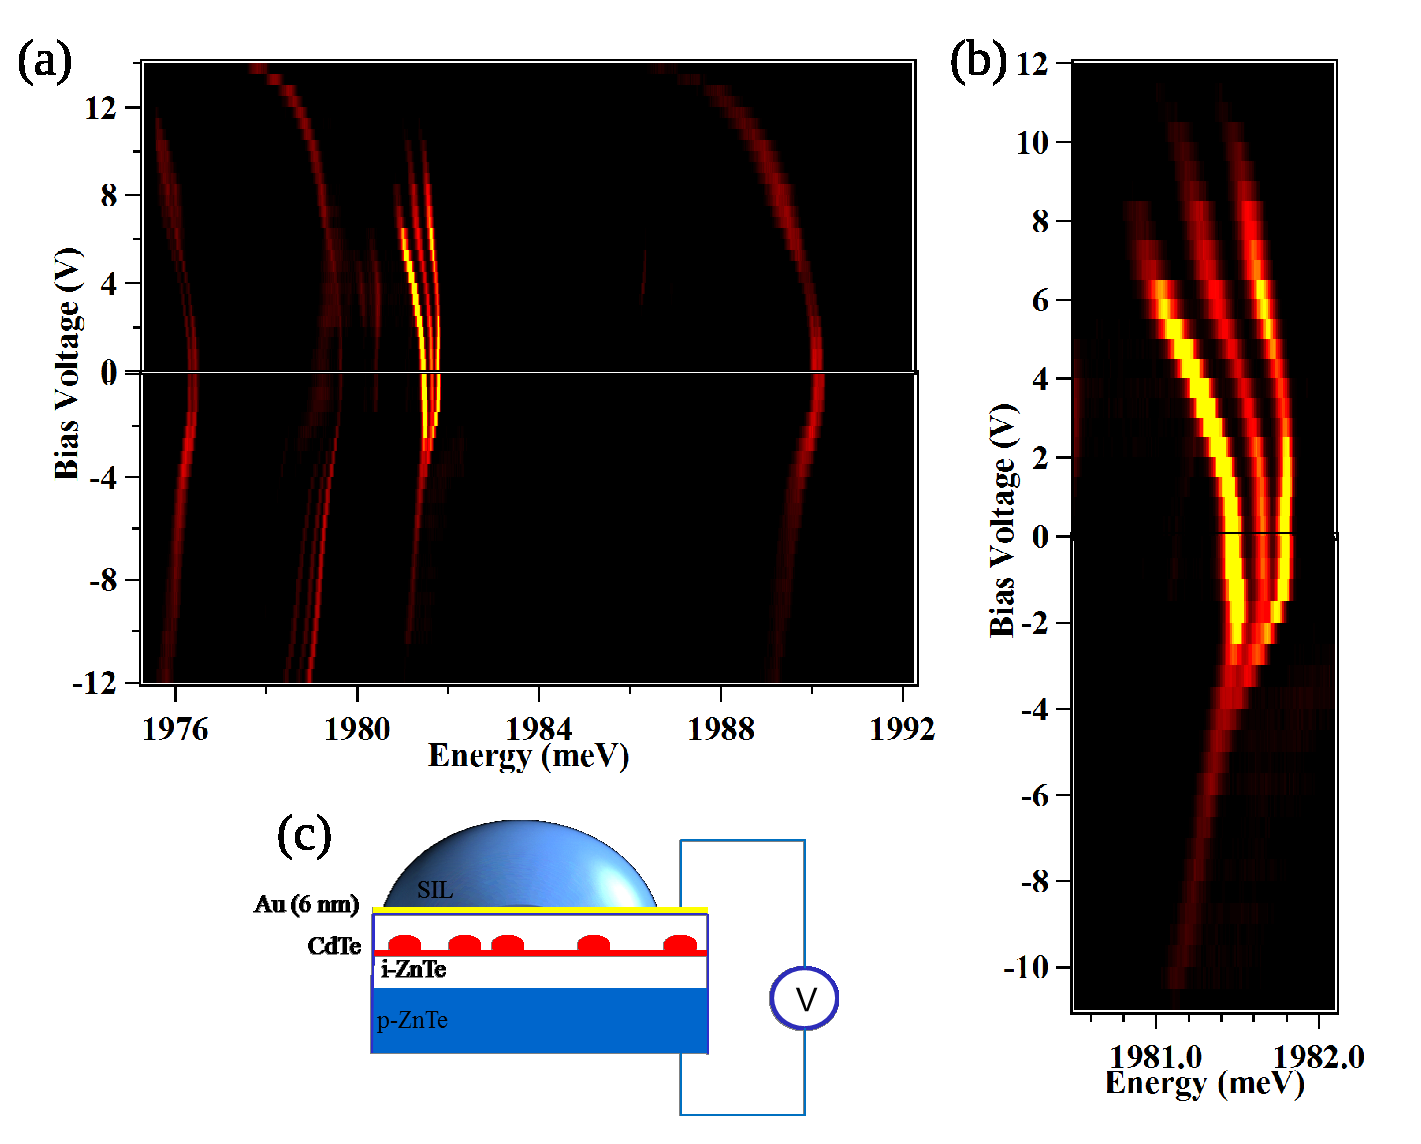
\includegraphics[width=12cm]{Pictures/EfieldX-Xc.eps}
	\end{center}
	\caption{(a) QD7 whole PL evolution under application of a bias voltage. (b) Zoom on X$^c$-Cr circular polarization PL intensity evolution under electric field. A strong stark shift is observed, as well as variation in the splitting. (c) Schema of a sample with a Schottky gate used to apply the bias voltage on the sample.}
	\label{CrSixPeaksEFieldX+}
	\end{figure}	
	
	To further investigate those dots, we study the evolution of their emission under bias voltage. The application of an electric field was realized via a sample with a Schottky gate in the same fashion than the one in Fig.~\ref{CrSixPeaksEFieldX+}(c). The resulting map is presented in Fig.~\ref{CrSixPeaksEFieldX+}(a). The first visible feature is the strong electric field dependency of the emission energy, more marked for X-Cr than for the X$^c$-Cr systems. The emission energy variation of the X-Cr complex occurs in a 2.9 meV range.
	
	There is another remarkable point on these maps, evidenced on the X$^+$-Cr complex on the Fig.~\ref{CrSixPeaksEFieldX+}(b): the splitting between each peak is changing with the applied electric field. The splitting between the high and low energy peaks varies from 0 meV for an applied bias voltage of -8V (no splitting) to 0.7 meV for 8V applied. This disappearance of the splitting for a certain bias voltage indicates that phenomena inducing an emission at three different energy can be tuned using an external electric field.

	\begin{figure}[h!]
	\begin{center}
		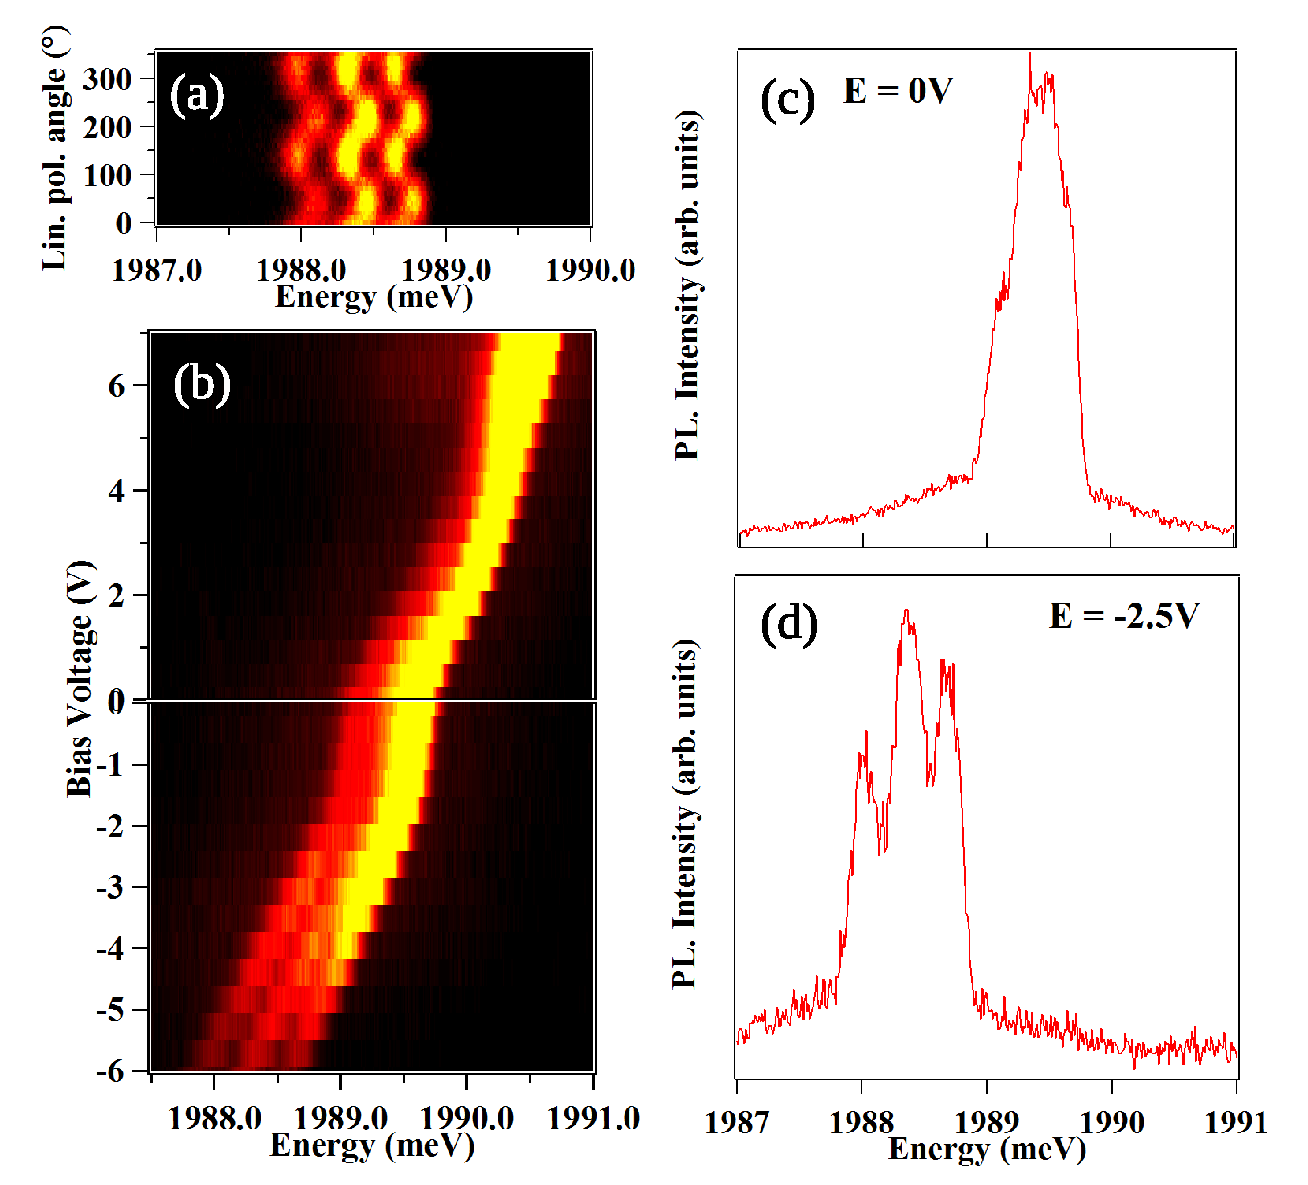
\includegraphics[width=12cm]{Pictures/SplitUnderEfiledXCr.eps}
	\end{center}
	\caption{All these measures were taken on QD8 X-Cr complex at low temperature. (a) PL intensity dependency in linear polarization. In order to have the best contrast, the map was taken at -2.5V bias voltage. (b) Circular PL intensity evolution in electric field. A splitting began to appear around -2V of applied bias voltage. (c)-(d) Circular PL for an applied bias voltage of, respectively, 0V and -2.5V.}
	\label{CrSixPeaksSplit}
	\end{figure}
		
	Fig.~\ref{CrSixPeaksSplit} shows that, using electric field, we can manipulate the splitting of any given charged state of the QD. For all positive bias voltage between 0V and 7V, X-Cr present a broad emission containing all six peaks in linear emission, as show on Fig.~\ref{CrSixPeaksSplit}(a). The emission then divide into three distinct peaks, starting to appear around -1V. This is evidenced on the the PL emission on Fig.~\ref{CrSixPeaksSplit}(d).
	
	\begin{figure}[h!]
	\begin{center}
		\includegraphics[width=14.9cm]{Pictures/CrCloseDot.png}
	\end{center}
	\caption{(a) Cr accessible charged states in ZnTe. (b)-(d) Illustration of the effect of a punctual charge on the wavefunction of an electron (red) and a hole (yellow) in a quantum dots.}
	\label{CrOutsideDot}
	\end{figure}
	
%	It is possible for the emission of a quantum dot to fluctuate between different energy under fluctuation of charge in the vicinity of a QD. This phenomena leads to a peak broadening~\cite{ChargeSpectFluct} as well as spectrum jumps. For the PL to jump between three emission energies, the charge fluctuation has to be able to take three distinct charge values.

	These complex appears with a high probability in sample with a high Cr concentration, for targeted Cr concentration above 0.10\% (see Sec.~\ref{SKGrowth}). None were found in sample for which the Cr was kept close. However, seeing there is no anti-crossing except the one expected for bright and dark exciton mixing, we can conclude that they are not caused by the interaction between carriers and Cr spins.
	
	We propose that those dots particular PLs are caused by Cr in the ZnTe barrier close to the dot. Cr is incorporated in ZnTe as Cr$^{2+}$, but, as shown on Fig.\ref{CrOutsideDot}(a), the Cr$^+$ and Cr$^{3+}$ states are in the gap and accessible~\cite{CrZnTe}, either by capturing an electron (Cr$^+$) or a hole (Cr$^{3+}$). Considering such a charge close to the QD, it can be viewed as a punctual one, since the dot is far bigger than the atom. The effect on the wave functions, presented in Fig.\ref{CrOutsideDot}(b)-(d), differs depending on the electrical charge of the Cr atom. Cr$^{2+}$ is the neutral state of Cr in ZnTe, sharing its outer shell electrons to bond with the atoms of the crystal. It is therefore the neutral position of the QD-Cr system. Capturing an electron, the Cr atom get a supplementary negative charge, and will thus attract more strongly the hole confined in the QD and repel the electron. The opposite happens when the Cr capture a hole.
	
	The electron is well confined in CdTe/ZnTe quantum dots and is thus not affected strongly by the presence of a punctual charge close to the QD. The hole, on the other hand, is only weakly confined in CdTe/ZnTe QDs. Its wavefunction is then more strongly affected by the charge variations of the Chromium. 
Because of this weak confinement, the hole wavefunction goes slightly out of the dot, and thus overlaps with the Cr atom. Its shape will then be strongly affected by change of charge of the Cr atom atom, being repel when the atom capture a hole, attracted when it capture an electron. This change in shape of the hole wavefunction affect the Coulomb interaction with the electron, and thus the emission energy of the exciton. The application of an electric field through the Schottky gate attract the hole toward the surface or the back of the sample, depending on the direction of the applied field. This attraction change the overlap of the hole wavefunction with the Cr atom, reducing it to zero for strong enough electric field. The emission energy is then not affected anymore by the charge variation of the Cr.

	These variations of a charge close to the dot would also explain the apparent splitting difference between the different excitonic complex (X, X$^+$, X$^-$ and X$^2$, see Fig.~\ref{CrSixPeaksMagOpt}). The binding energies of the different charged species and of the biexciton decreases when the electric field increases, due to the difference of polarity between the hole and the exciton~\cite{BesombesEfieldExciton}. This lead to smaller jump in energy when there is a charge close to the dot, and thus a smaller apparent splitting.

%	This weak confinement also mean that the wavefunction goes slightly out of the dot, and thus the overlap with the Cr atom might exist for the hole, even if the atom is not in the QD. The slight overlap is enough to cause the splitting of the exciton emission PL via the exchange interaction, without the Cr being affected by the dot. When the atom get a positive charge, it will repel the hole, reducing the overlap until none remain, killing the splitting of the emission. The opposite happens when the Cr capture an electron, attracting the hole and improving the overlap. The overlap can also be affected by the application of a magnetic field through the Schottky gate, which will change the  wavefunctions shape and the probability for the Cr atom to be in a given charge state.
	
%	The charge variation of the Cr is of the value of the elementary charge. Considering a pure coulomb interaction between two punctual charges, for a charge at 5nm of the dot, its effect is of the same order of magnitude than the hole-Cr exchange interaction. In order to have a significant effect on the dot PL, the Cr has then to be close to it, not more than a few nanometres away. 
	
	This hypothesis is currently tested, along with the capacity for the Cr to diffuse outside the quantum dots layer during the MBE growth.
	
	\section*{Conclusion}
	
%	For the first time, a single Cr atom was embedded inside a II-VI quantum dot. We were then able to probe it optically. Such a system presents a characteristic three peak emission, along with the emission of a dark state on the low energy side. The action of the magnetic anisotropy, splitting the Cr spin states according to $D_0 S_z^2$, is strong enough to keep the $S_z = \pm2$ level to be thermally populated, and thus they do not present luminescence. The QDs show a good spin conversation during the exciton lifetime inside the dot, thanks to the effective magnetic field created by the Cr spin. Magneto-optics confirm the chosen energy structure and gives us the possibility to deduce the magnitude of several of the quantum dot parameters. We used the model to simulate the emission of QD with different parameters, and proposed an explanation to the absence of high anisotropy QDs in the one we probed. Some dots seems to correspond to these high anisotropy QDs, but they show no sign of magnetic atom inside them under further investigation. We finished proposing a possible explanation for those dots, supposing the presence of Cr atoms in the ZnTe barrier.
	
	For the first time, a single Cr atom was embedded inside a II-VI quantum dot and its spin was probed optically. It presents a characteristic three peaks structure under optical probing. The splitting caused by the magnetic anisotropy is strong enough to keep the states $S_z = \pm2$ to be thermally populated. The central peaks may be split in low symmetry quantum dot, and a fourth peak, corresponding to a dark state may appear on the low energy side. Magneto-optic experiments confirm this energy structure and show several anti-crossing characteristic from a Cr doped quantum dots, giving us possibility to extract parameters of the dot. They also evidence that the h-Cr coupling is anti-ferromagnetic, contrary to what was suggested in the literature. 
	
	Having successfully inserted and probed single Cr atom spins in CdTe/ZnTe quantum dots, it is now important to study how this system evolve in time. An important step for further use of the system is the possibility to prepare the Cr spin in a chosen state, and then control it. This is what we propose to study in the next chapter.

\printbibliography

\end{document}
